
\documentclass{article}
\usepackage{graphicx}
\usepackage[margin=1in]{geometry}
\usepackage{caption}
\title{Radar Chart Summary}
\date{}
\begin{document}
\maketitle

\begin{figure}[h!]
  \centering
  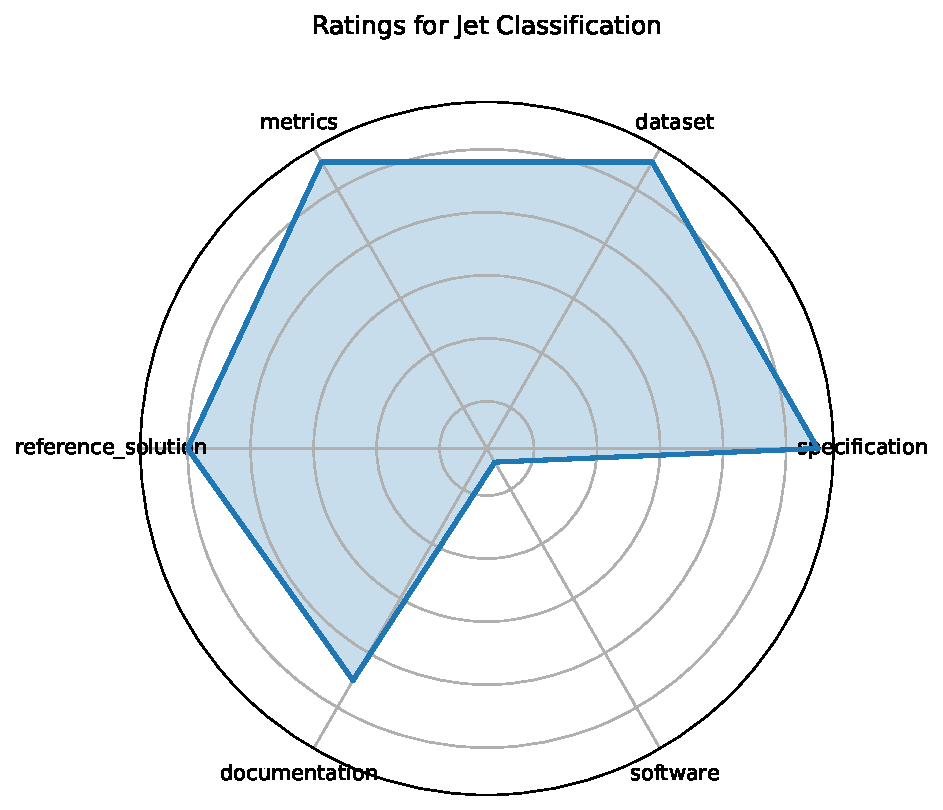
\includegraphics[width=0.7\textwidth]{Jet Classification_radar.pdf}
  \caption{Jet Classification}
\end{figure}

\begin{figure}[h!]
  \centering
  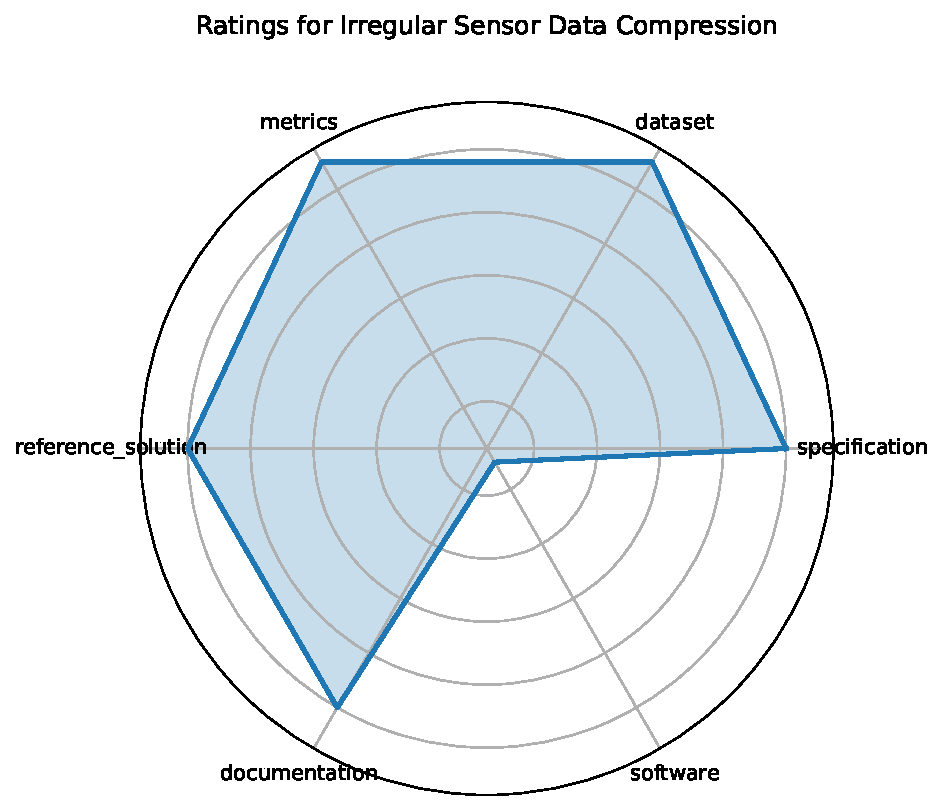
\includegraphics[width=0.7\textwidth]{Irregular Sensor Data Compression_radar.pdf}
  \caption{Irregular Sensor Data Compression}
\end{figure}

\begin{figure}[h!]
  \centering
  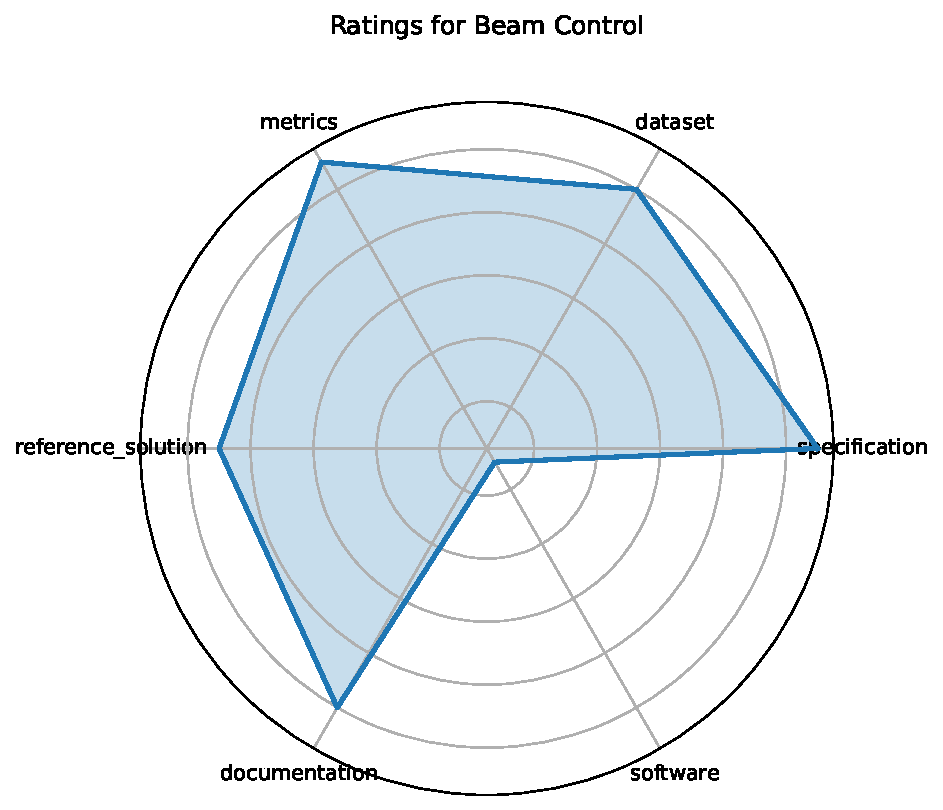
\includegraphics[width=0.7\textwidth]{Beam Control_radar.pdf}
  \caption{Beam Control}
\end{figure}

\begin{figure}[h!]
  \centering
  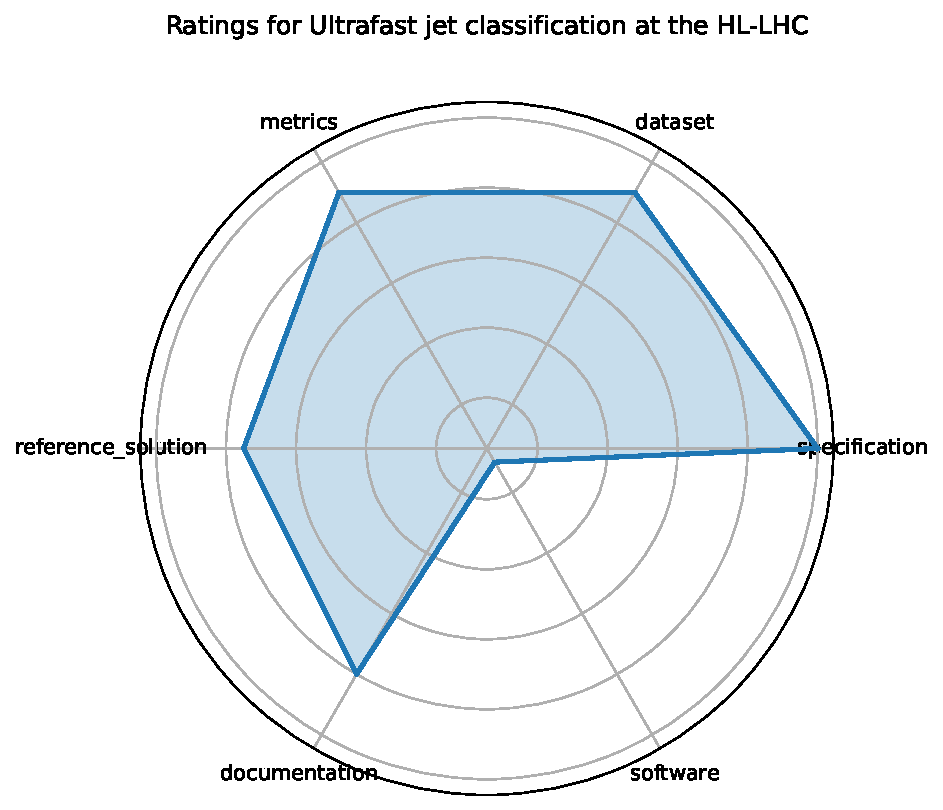
\includegraphics[width=0.7\textwidth]{Ultrafast jet classification at the HL-LHC_radar.pdf}
  \caption{Ultrafast jet classification at the HL-LHC}
\end{figure}

\begin{figure}[h!]
  \centering
  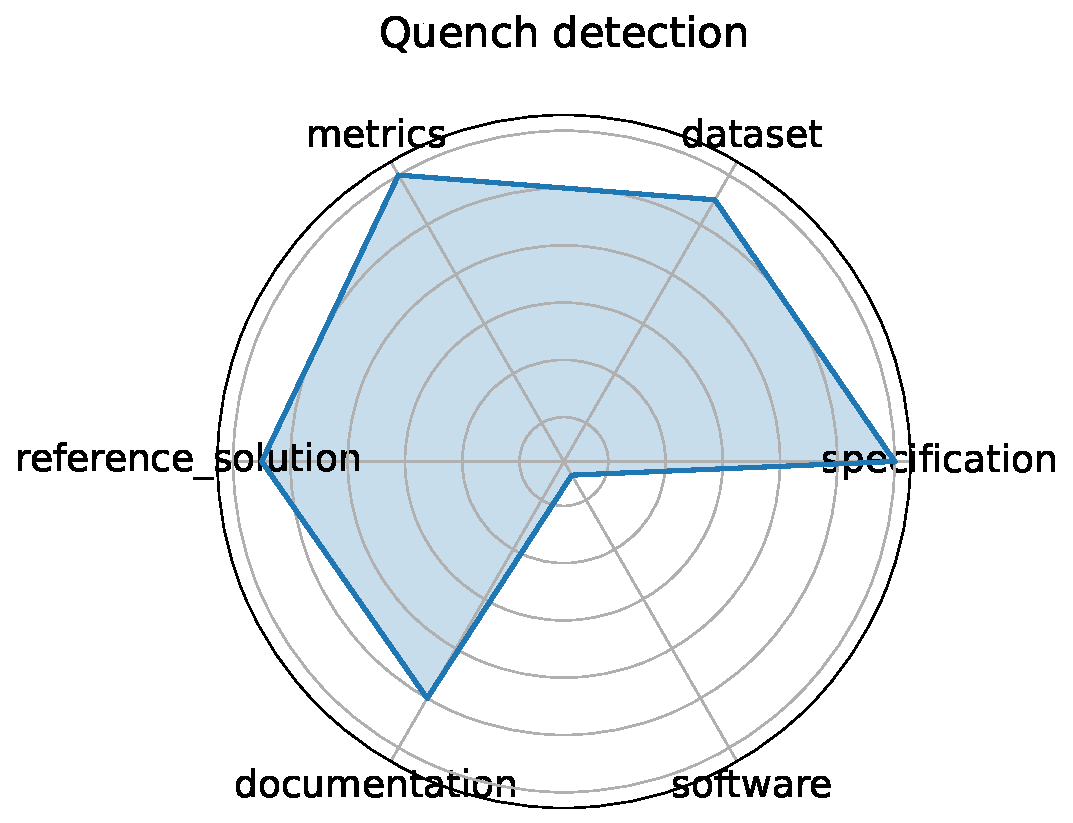
\includegraphics[width=0.7\textwidth]{Quench detection_radar.pdf}
  \caption{Quench detection}
\end{figure}

\begin{figure}[h!]
  \centering
  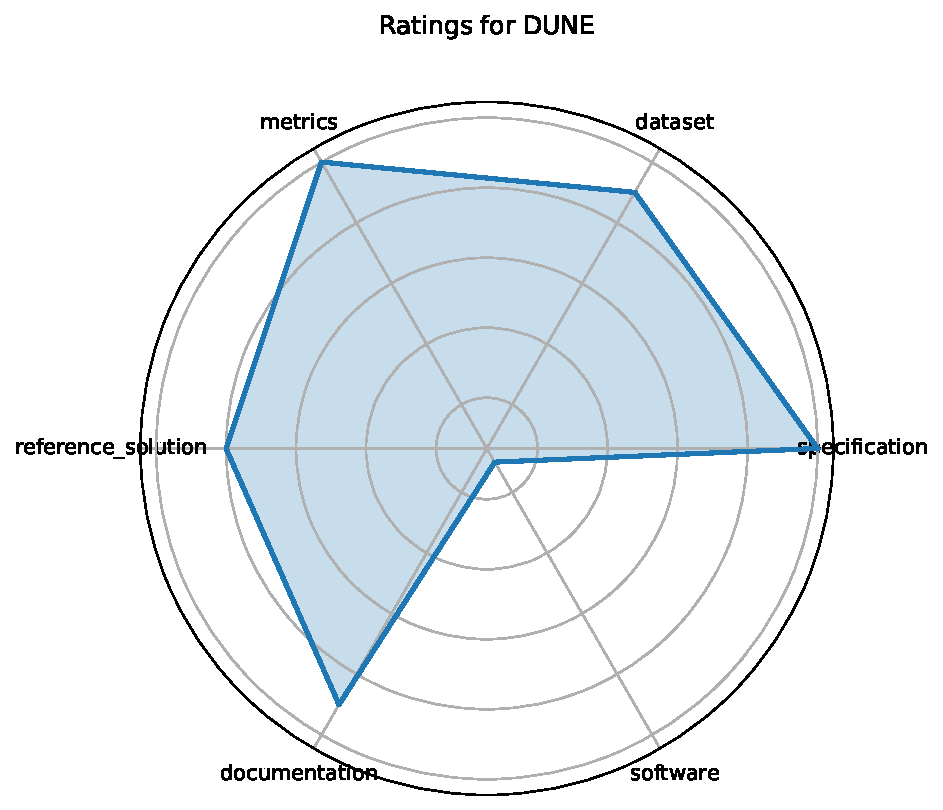
\includegraphics[width=0.7\textwidth]{DUNE_radar.pdf}
  \caption{DUNE}
\end{figure}

\begin{figure}[h!]
  \centering
  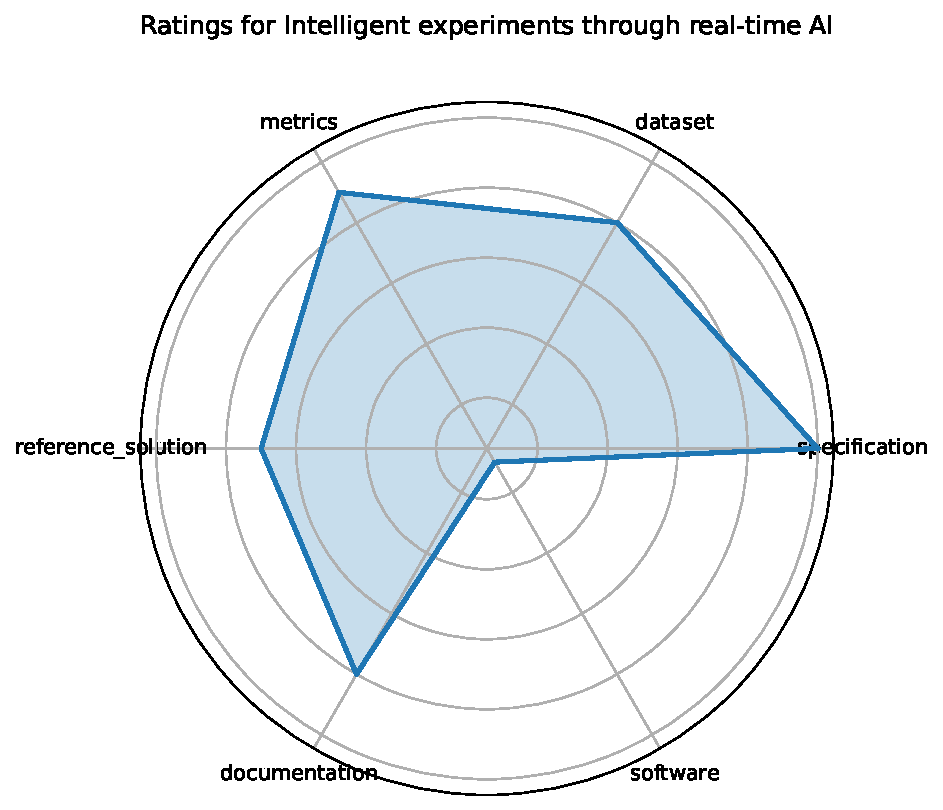
\includegraphics[width=0.7\textwidth]{Intelligent experiments through real-time AI_radar.pdf}
  \caption{Intelligent experiments through real-time AI}
\end{figure}

\begin{figure}[h!]
  \centering
  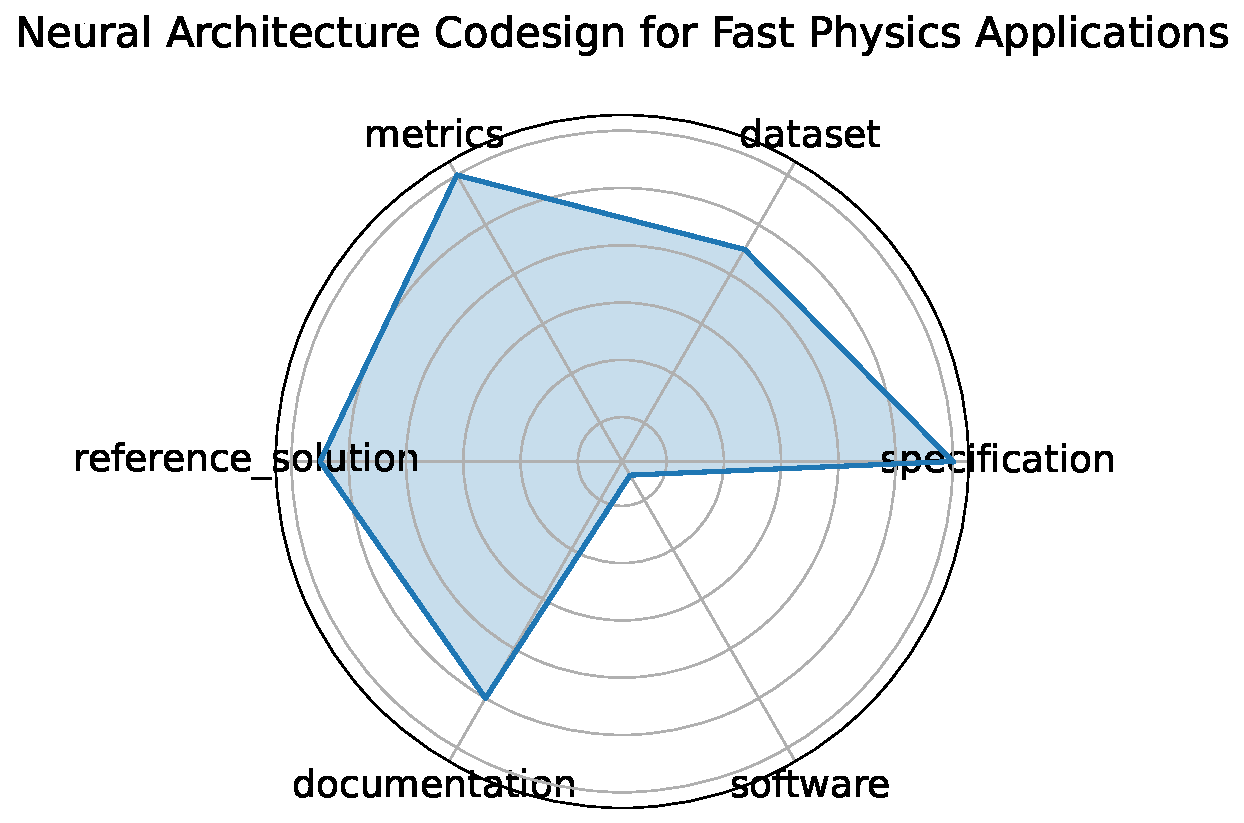
\includegraphics[width=0.7\textwidth]{Neural Architecture Codesign for Fast Physics Applications_radar.pdf}
  \caption{Neural Architecture Codesign for Fast Physics Applications}
\end{figure}

\begin{figure}[h!]
  \centering
  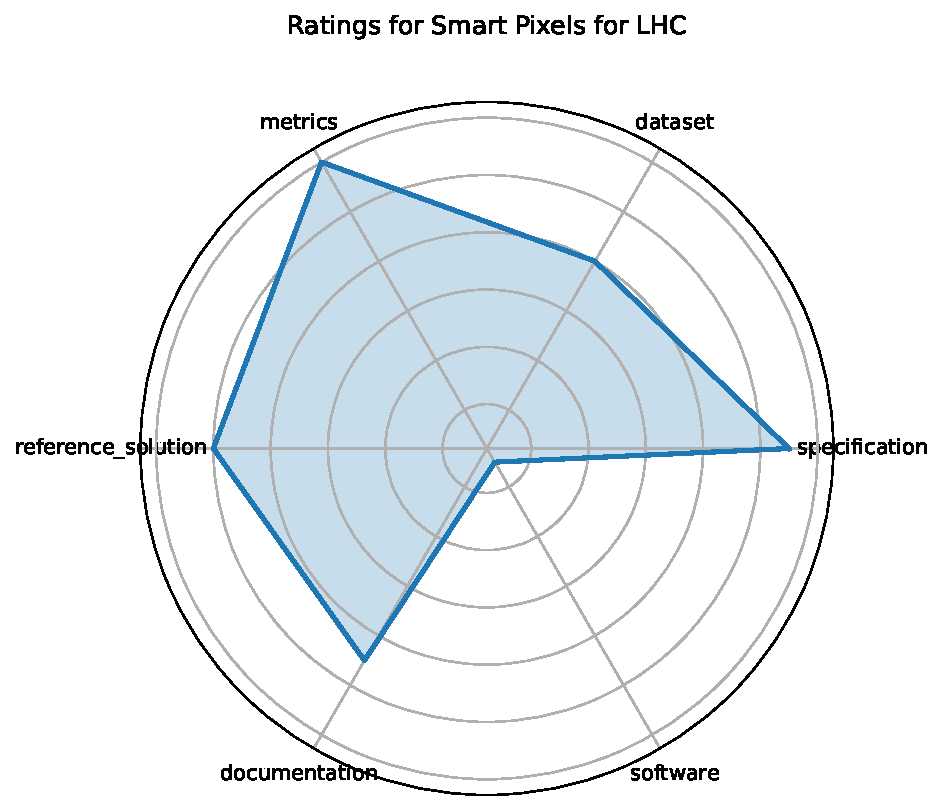
\includegraphics[width=0.7\textwidth]{Smart Pixels for LHC_radar.pdf}
  \caption{Smart Pixels for LHC}
\end{figure}

\begin{figure}[h!]
  \centering
  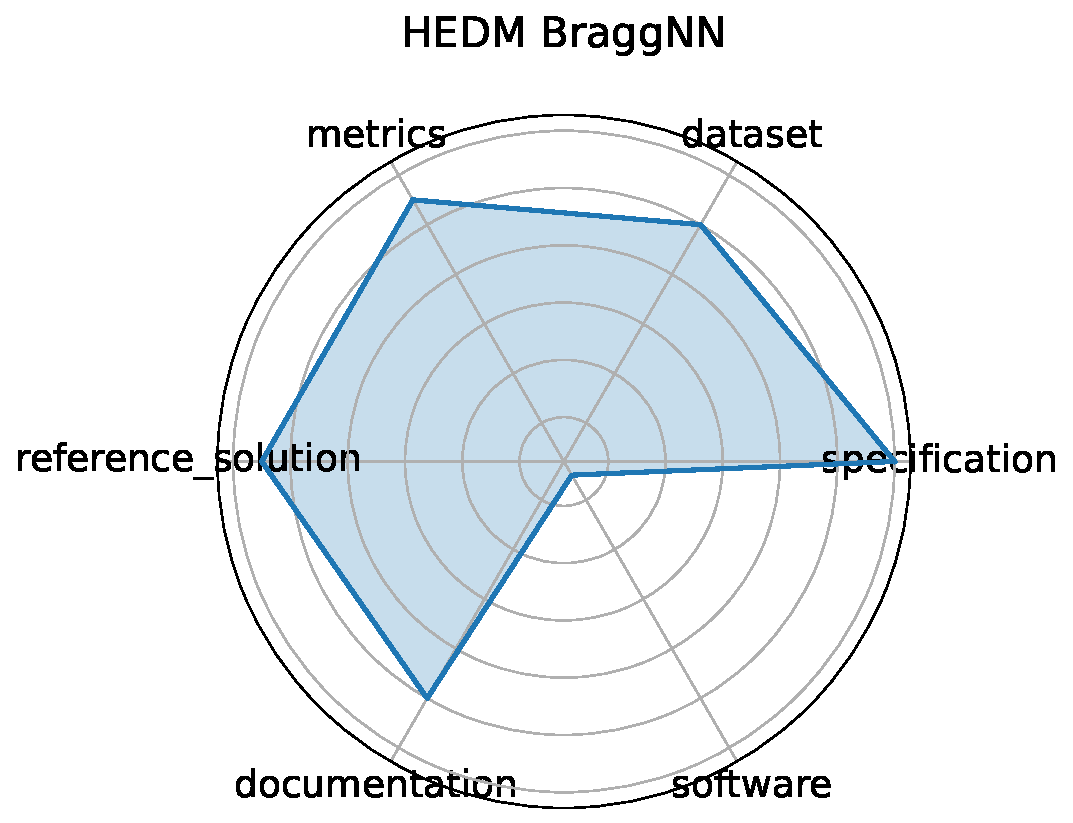
\includegraphics[width=0.7\textwidth]{HEDM BraggNN_radar.pdf}
  \caption{HEDM BraggNN}
\end{figure}

\begin{figure}[h!]
  \centering
  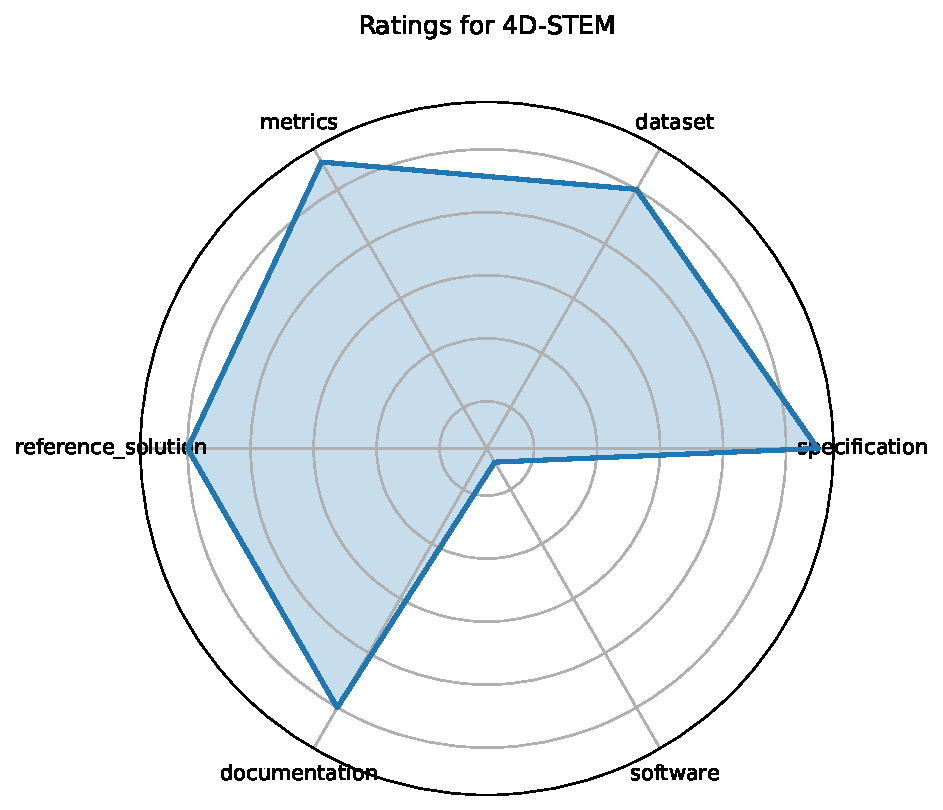
\includegraphics[width=0.7\textwidth]{4D-STEM_radar.pdf}
  \caption{4D-STEM}
\end{figure}

\begin{figure}[h!]
  \centering
  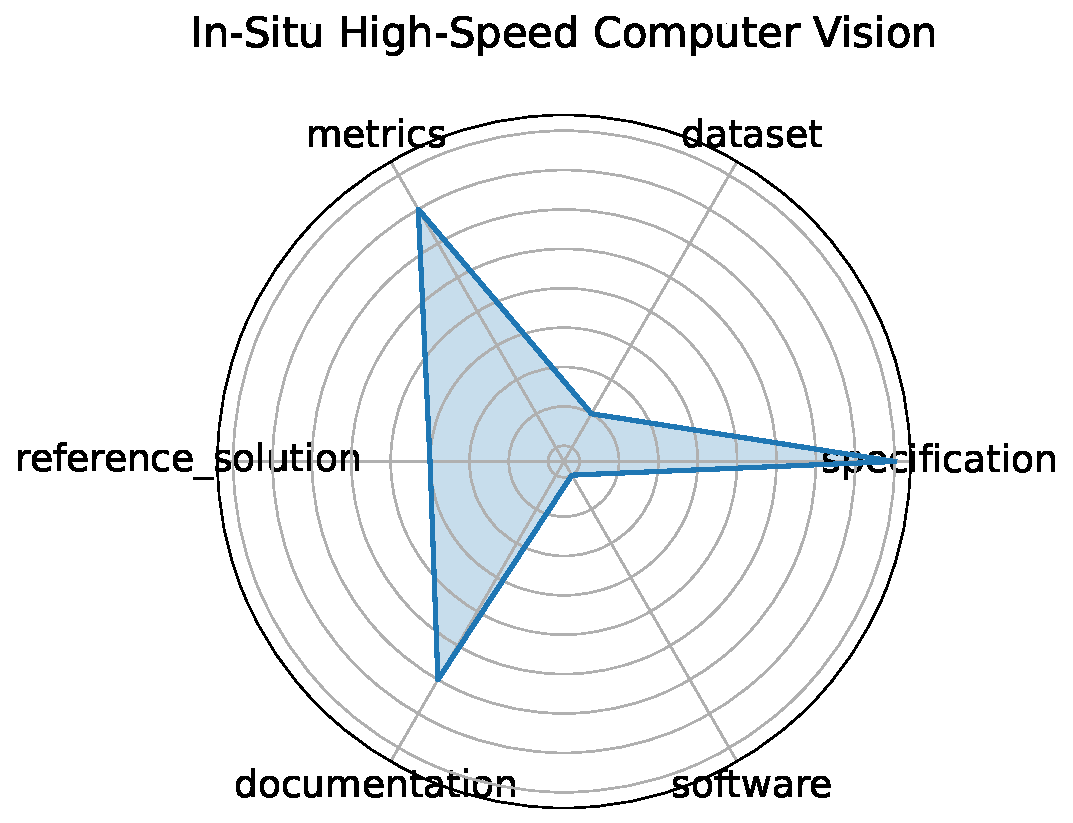
\includegraphics[width=0.7\textwidth]{In-Situ High-Speed Computer Vision_radar.pdf}
  \caption{In-Situ High-Speed Computer Vision}
\end{figure}

\begin{figure}[h!]
  \centering
  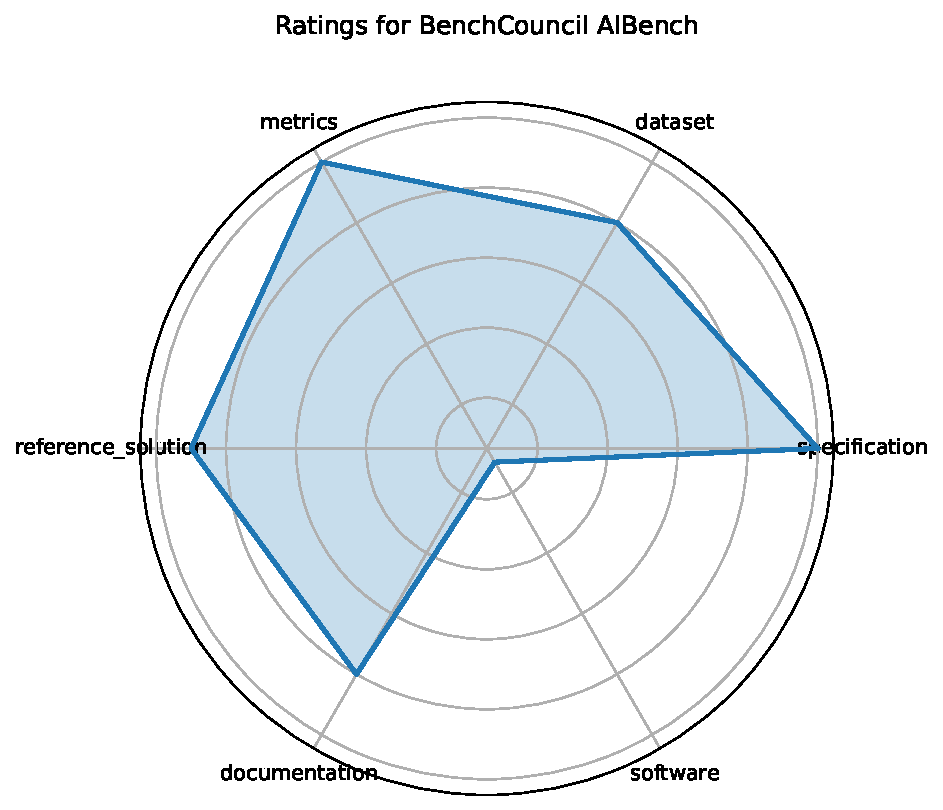
\includegraphics[width=0.7\textwidth]{BenchCouncil AIBench_radar.pdf}
  \caption{BenchCouncil AIBench}
\end{figure}

\begin{figure}[h!]
  \centering
  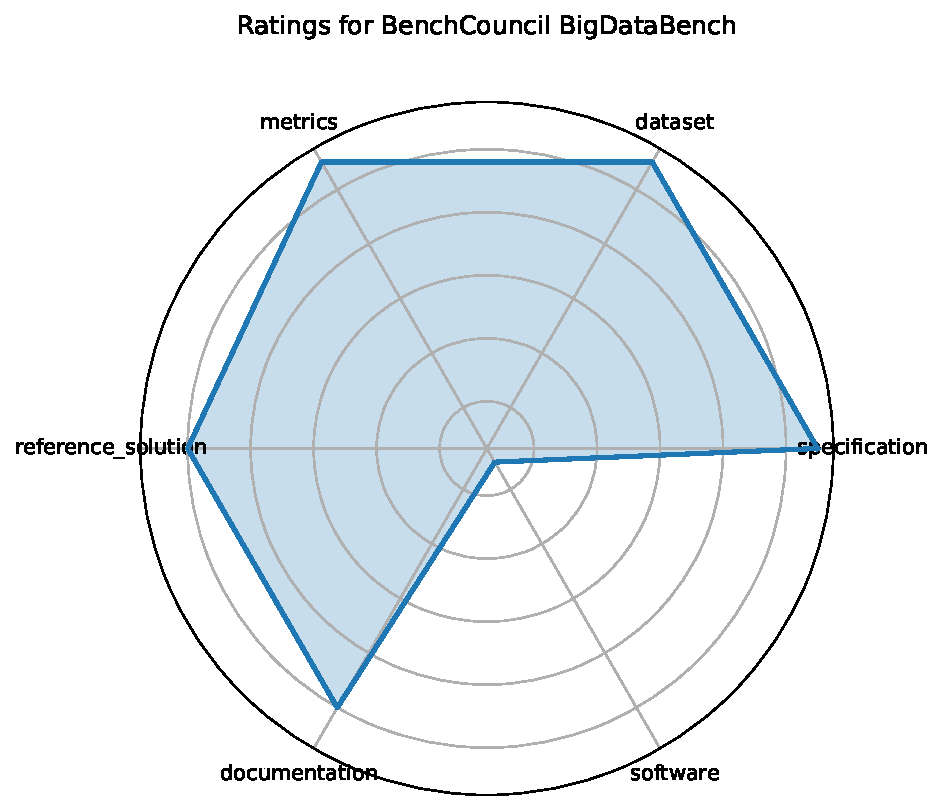
\includegraphics[width=0.7\textwidth]{BenchCouncil BigDataBench_radar.pdf}
  \caption{BenchCouncil BigDataBench}
\end{figure}

\begin{figure}[h!]
  \centering
  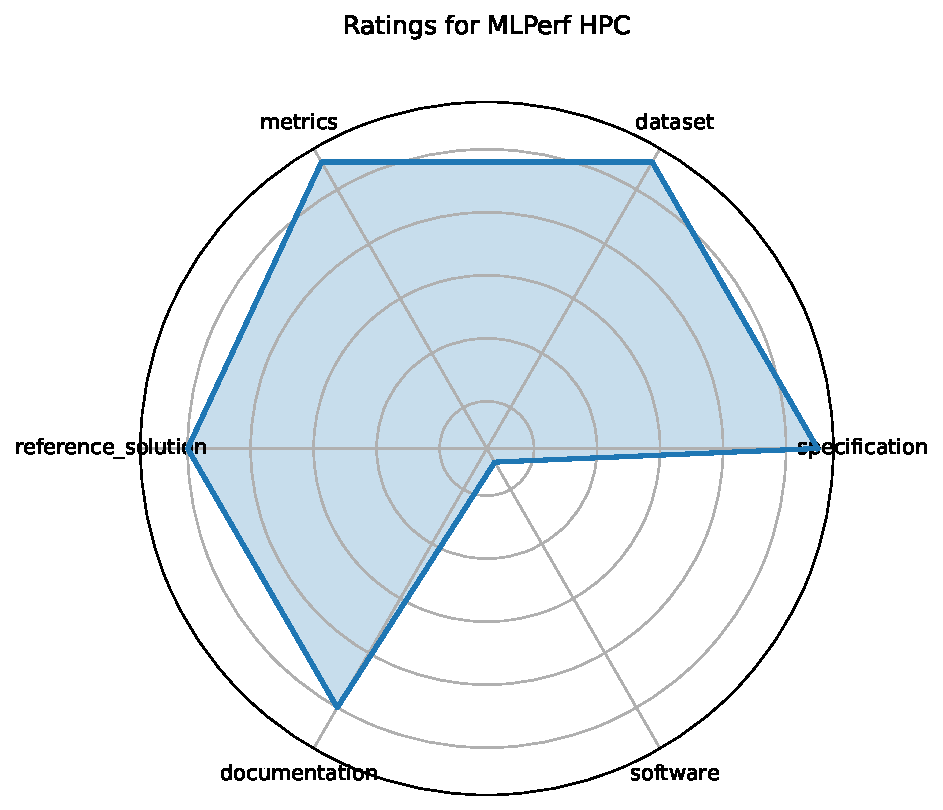
\includegraphics[width=0.7\textwidth]{MLPerf HPC_radar.pdf}
  \caption{MLPerf HPC}
\end{figure}

\begin{figure}[h!]
  \centering
  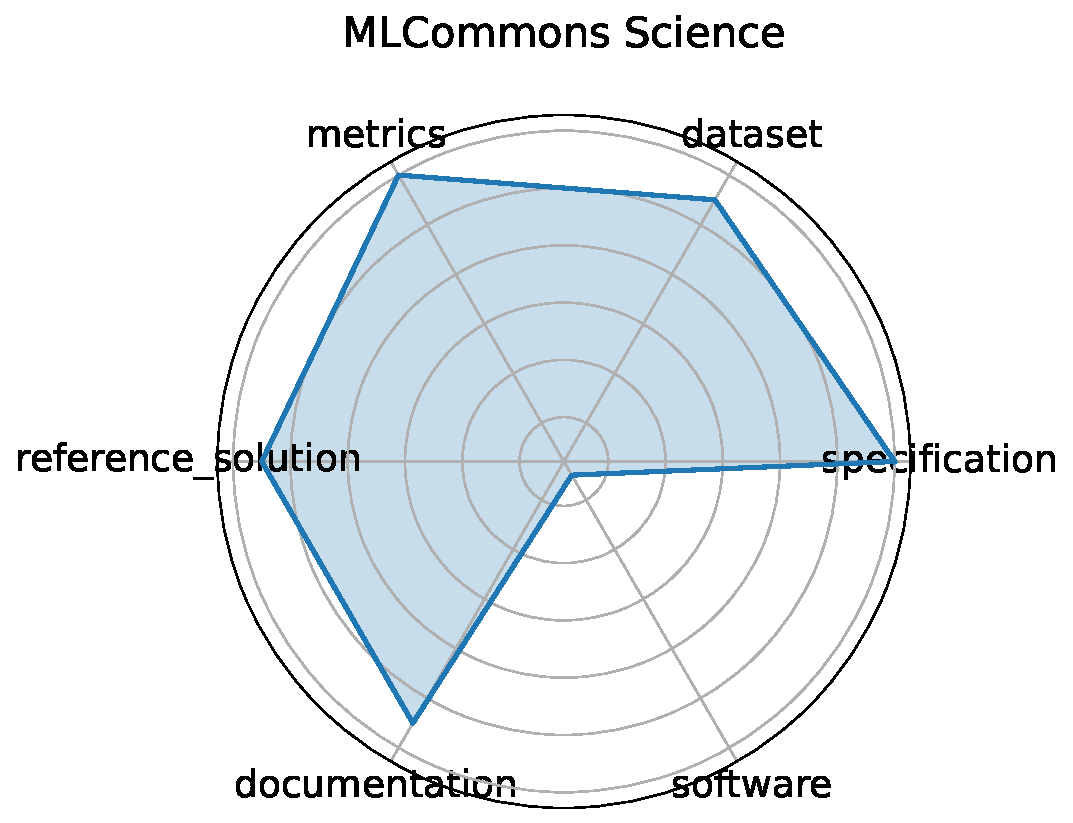
\includegraphics[width=0.7\textwidth]{MLCommons Science_radar.pdf}
  \caption{MLCommons Science}
\end{figure}

\begin{figure}[h!]
  \centering
  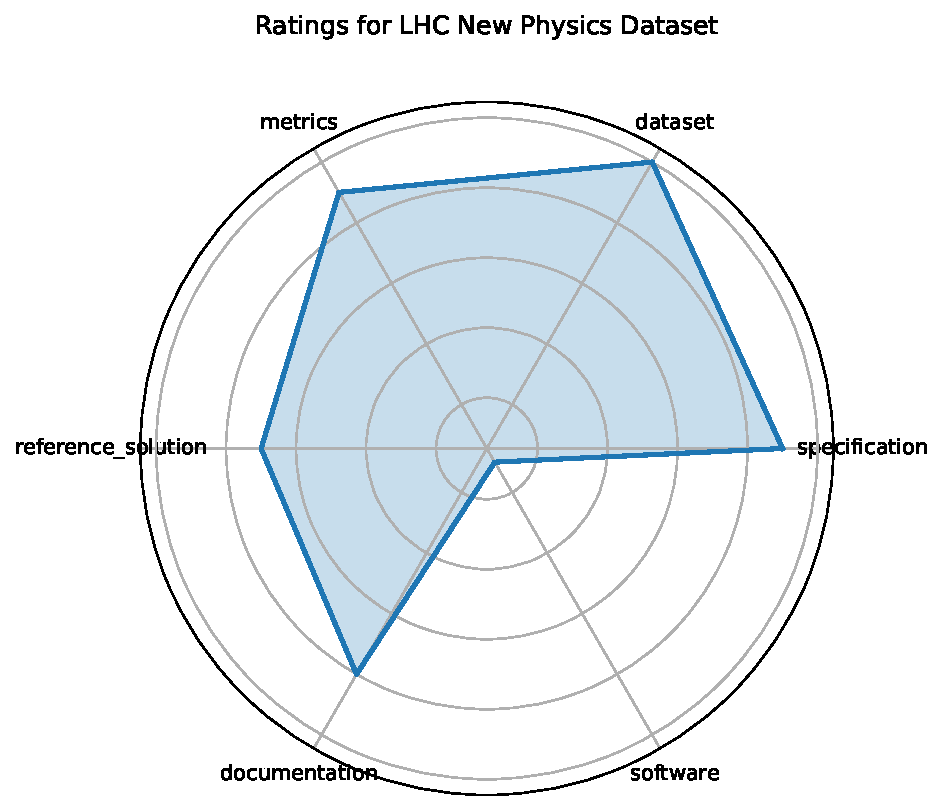
\includegraphics[width=0.7\textwidth]{LHC New Physics Dataset_radar.pdf}
  \caption{LHC New Physics Dataset}
\end{figure}

\begin{figure}[h!]
  \centering
  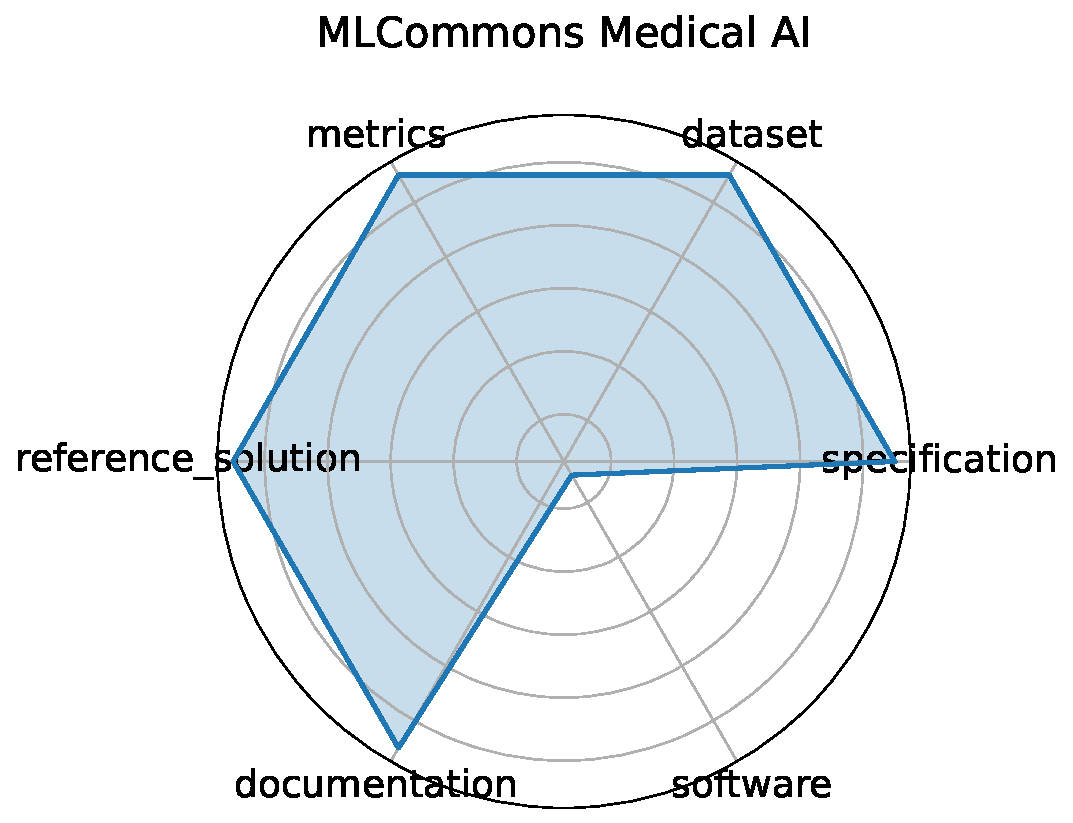
\includegraphics[width=0.7\textwidth]{MLCommons Medical AI_radar.pdf}
  \caption{MLCommons Medical AI}
\end{figure}

\begin{figure}[h!]
  \centering
  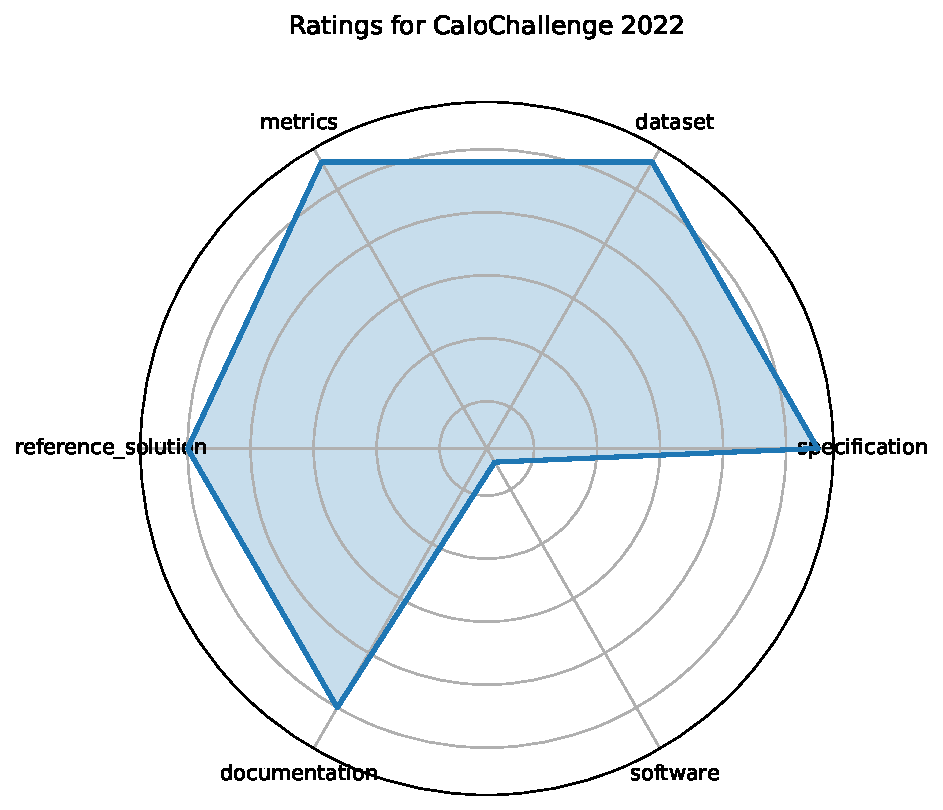
\includegraphics[width=0.7\textwidth]{CaloChallenge 2022_radar.pdf}
  \caption{CaloChallenge 2022}
\end{figure}

\begin{figure}[h!]
  \centering
  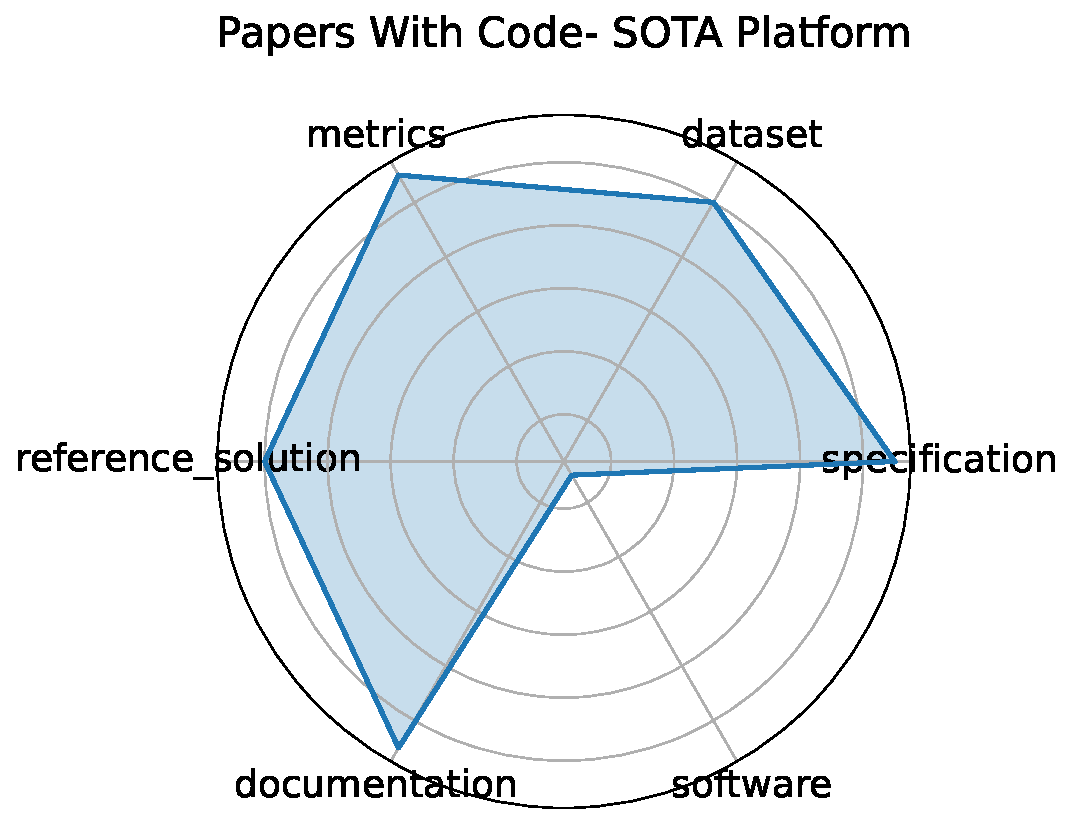
\includegraphics[width=0.7\textwidth]{Papers With Code- SOTA Platform_radar.pdf}
  \caption{Papers With Code- SOTA Platform}
\end{figure}

\begin{figure}[h!]
  \centering
  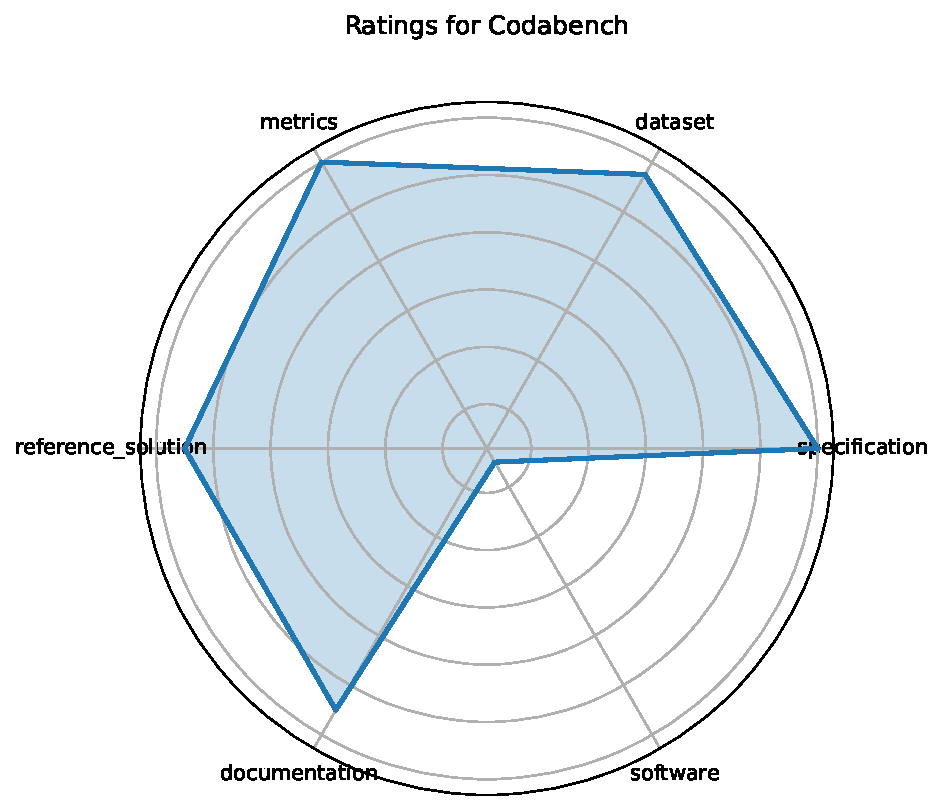
\includegraphics[width=0.7\textwidth]{Codabench_radar.pdf}
  \caption{Codabench}
\end{figure}

\begin{figure}[h!]
  \centering
  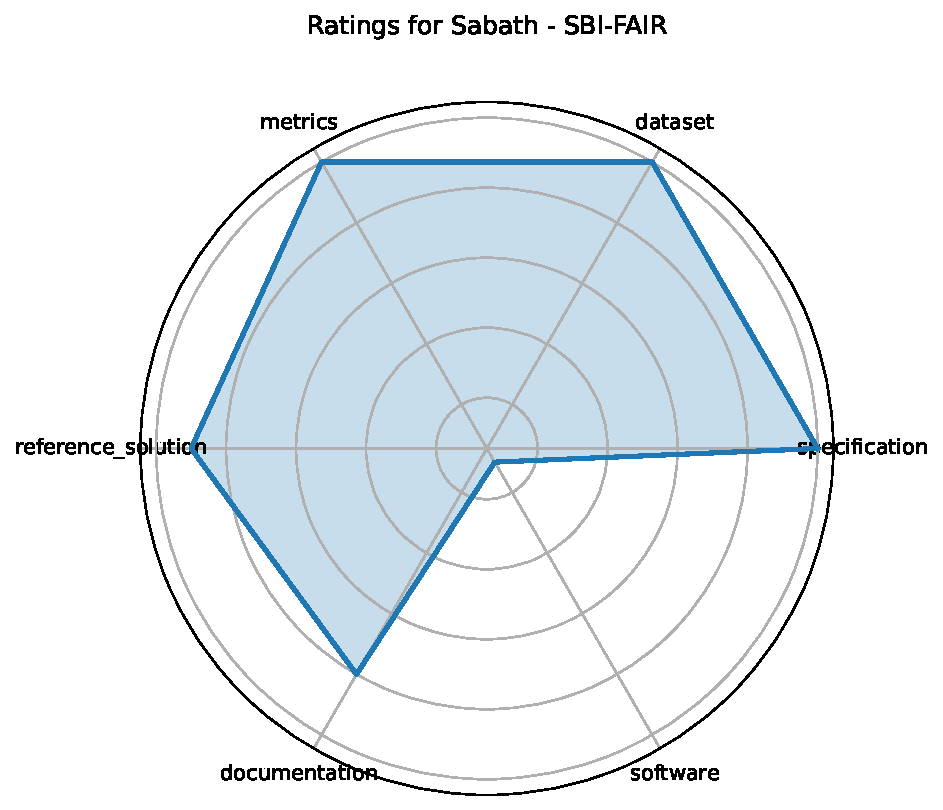
\includegraphics[width=0.7\textwidth]{Sabath - SBI-FAIR_radar.pdf}
  \caption{Sabath - SBI-FAIR}
\end{figure}

\begin{figure}[h!]
  \centering
  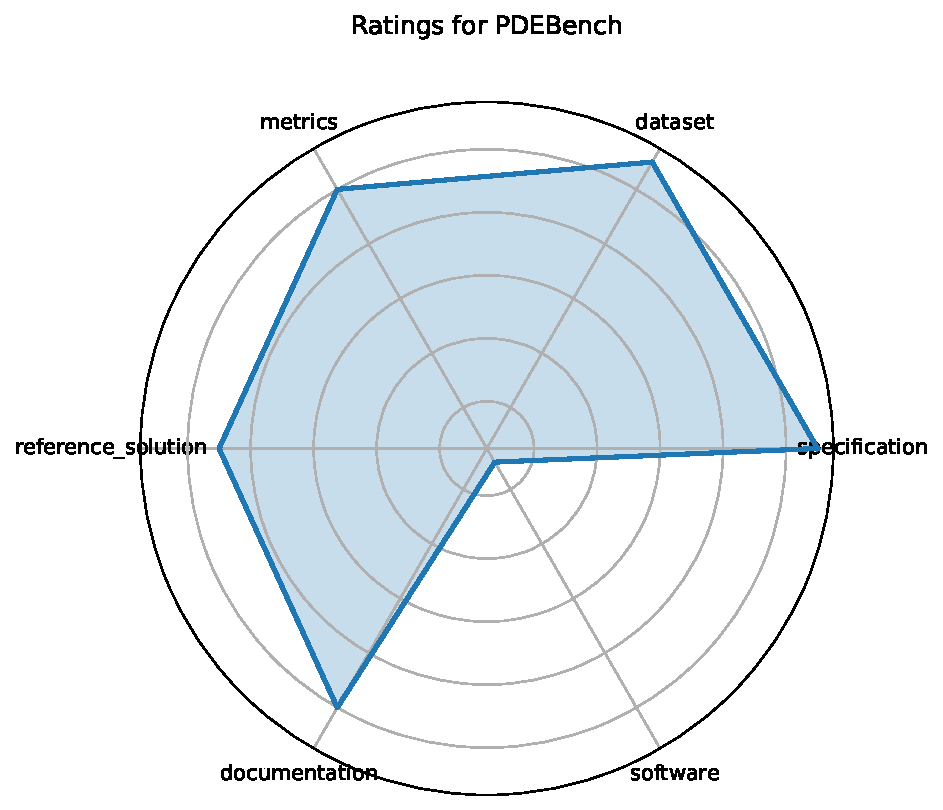
\includegraphics[width=0.7\textwidth]{PDEBench_radar.pdf}
  \caption{PDEBench}
\end{figure}

\begin{figure}[h!]
  \centering
  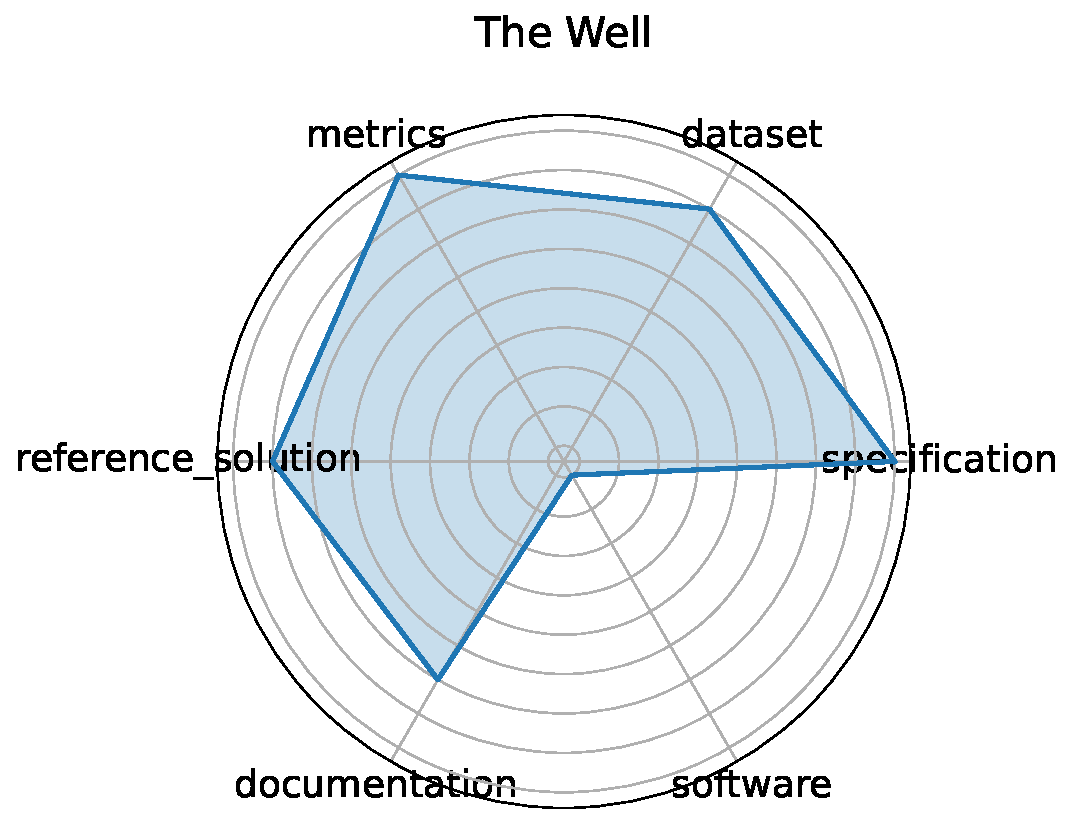
\includegraphics[width=0.7\textwidth]{The Well_radar.pdf}
  \caption{The Well}
\end{figure}

\begin{figure}[h!]
  \centering
  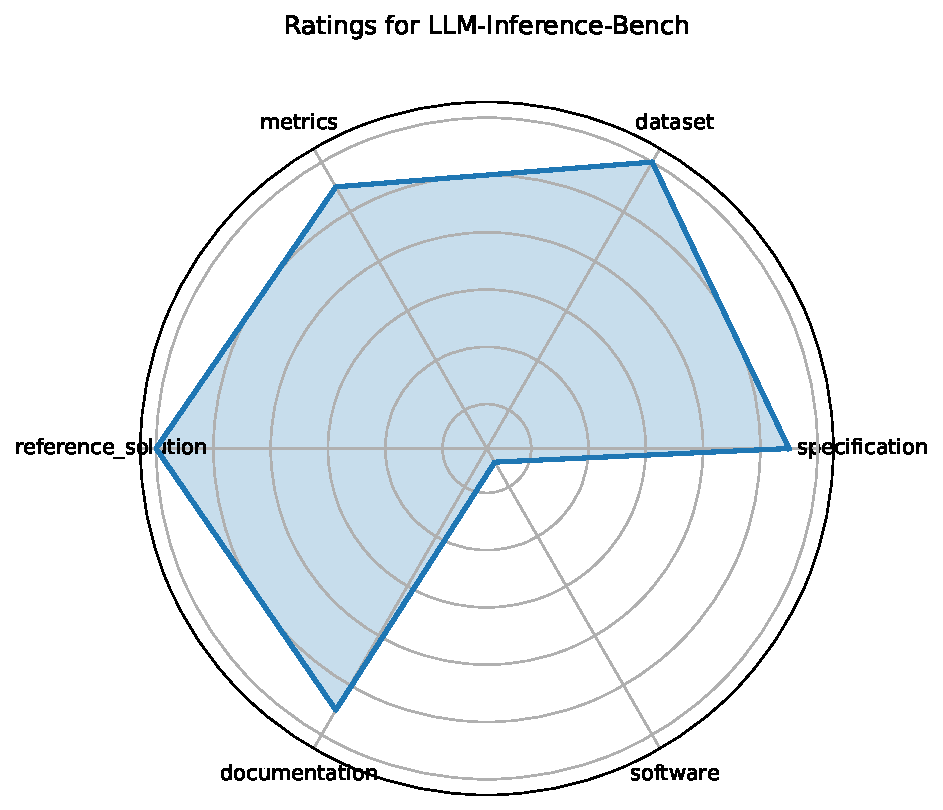
\includegraphics[width=0.7\textwidth]{LLM-Inference-Bench_radar.pdf}
  \caption{LLM-Inference-Bench}
\end{figure}

\begin{figure}[h!]
  \centering
  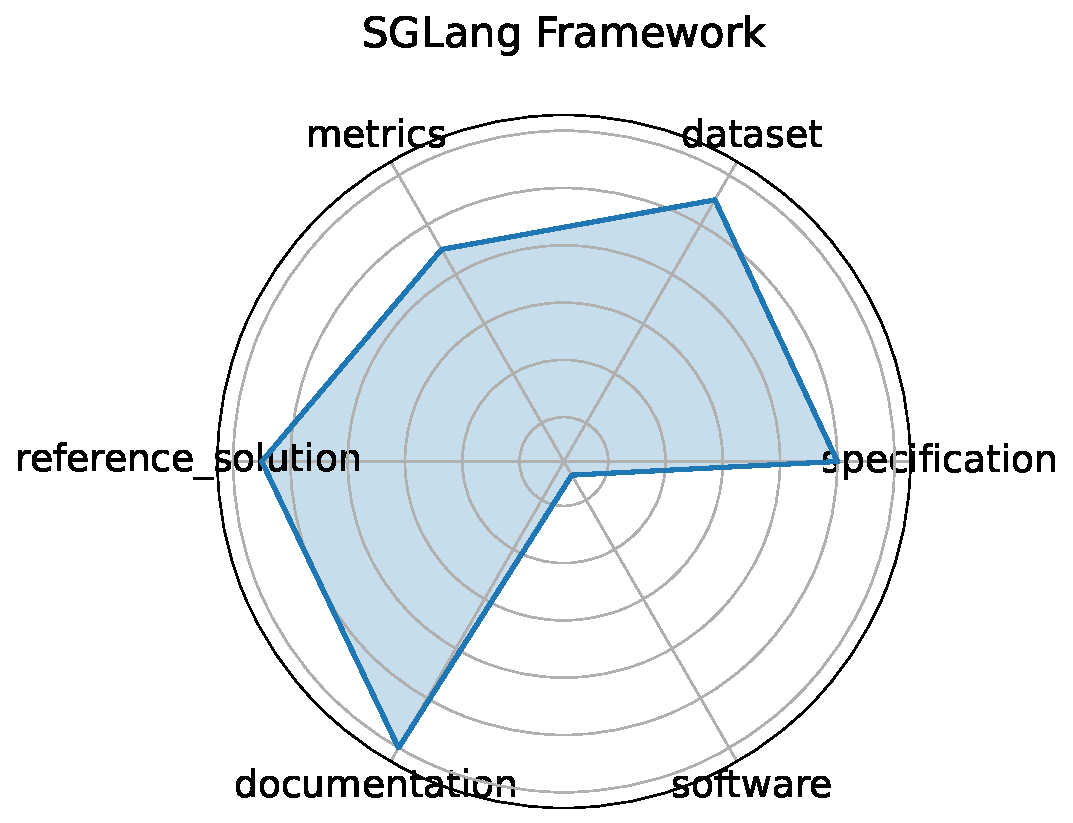
\includegraphics[width=0.7\textwidth]{SGLang Framework_radar.pdf}
  \caption{SGLang Framework}
\end{figure}

\begin{figure}[h!]
  \centering
  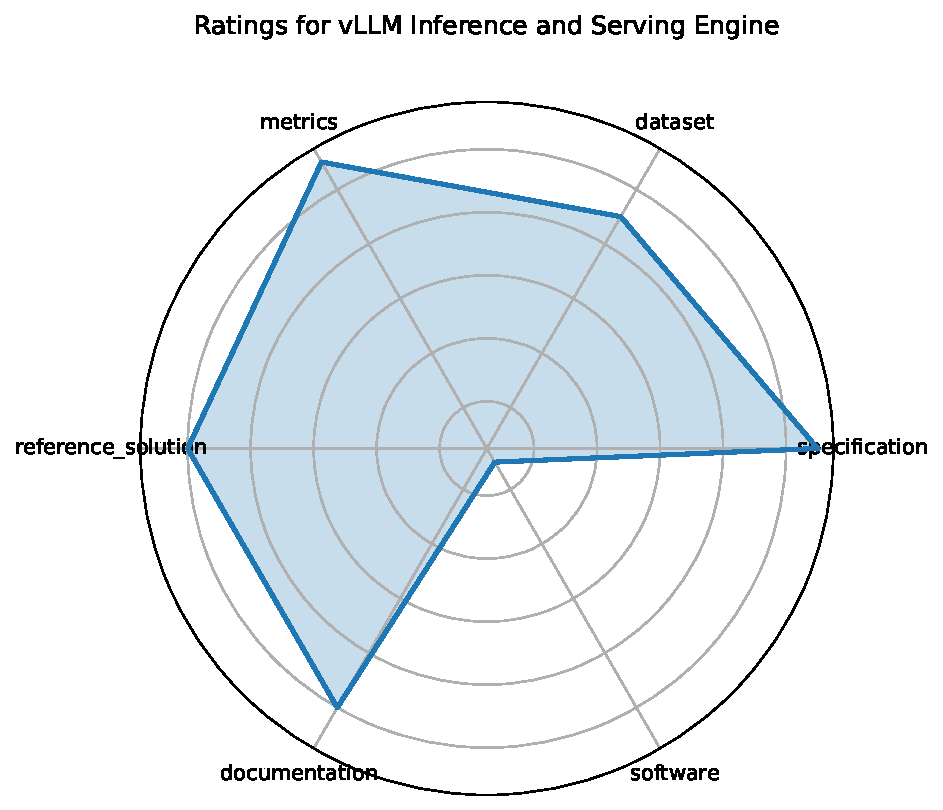
\includegraphics[width=0.7\textwidth]{vLLM Inference and Serving Engine_radar.pdf}
  \caption{vLLM Inference and Serving Engine}
\end{figure}

\begin{figure}[h!]
  \centering
  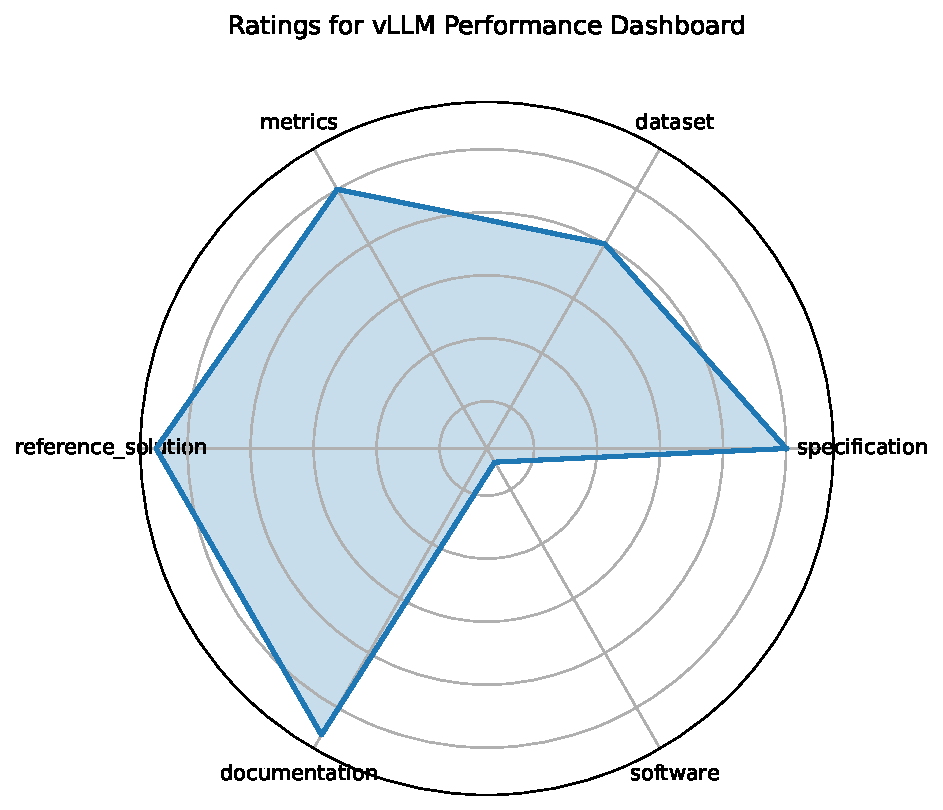
\includegraphics[width=0.7\textwidth]{vLLM Performance Dashboard_radar.pdf}
  \caption{vLLM Performance Dashboard}
\end{figure}

\begin{figure}[h!]
  \centering
  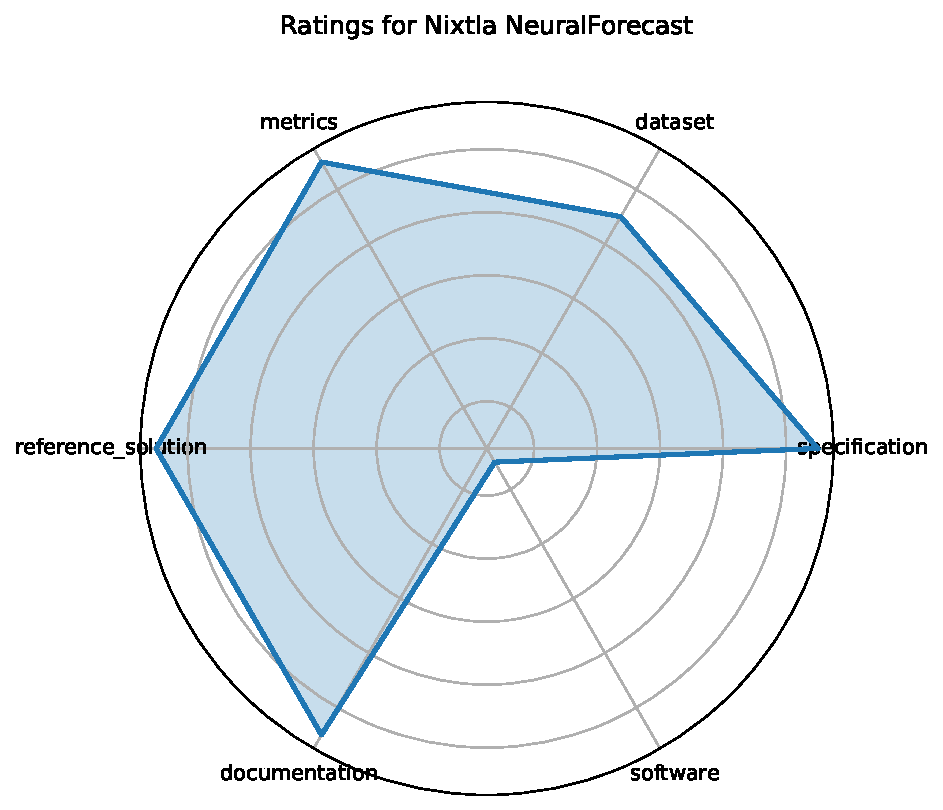
\includegraphics[width=0.7\textwidth]{Nixtla NeuralForecast_radar.pdf}
  \caption{Nixtla NeuralForecast}
\end{figure}

\begin{figure}[h!]
  \centering
  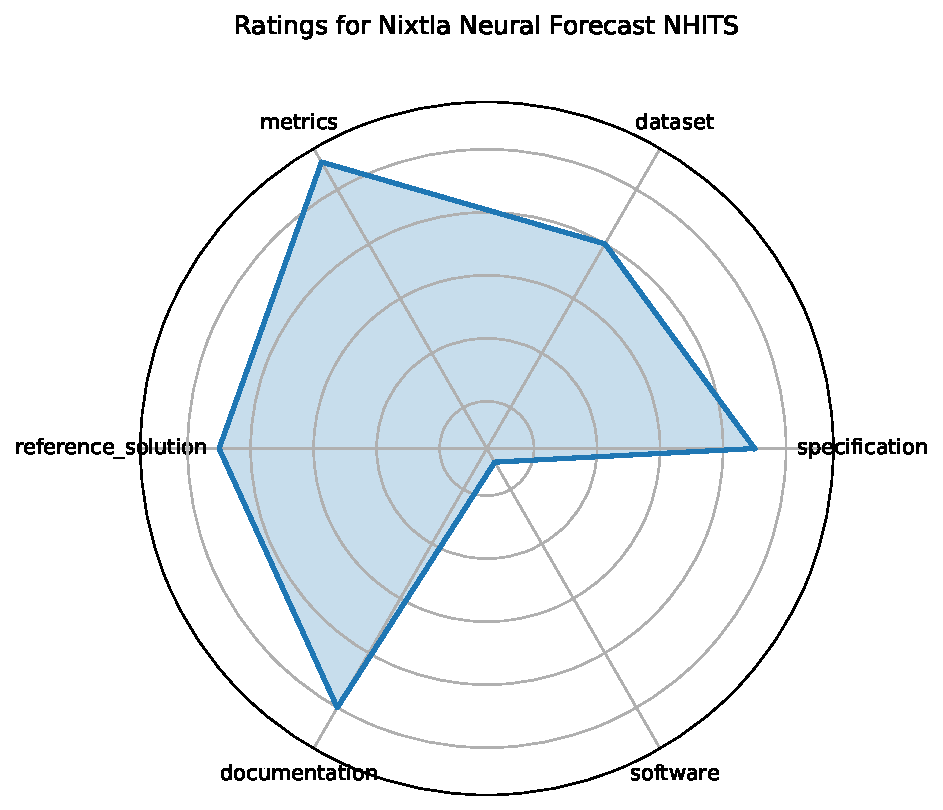
\includegraphics[width=0.7\textwidth]{Nixtla Neural Forecast NHITS_radar.pdf}
  \caption{Nixtla Neural Forecast NHITS}
\end{figure}

\begin{figure}[h!]
  \centering
  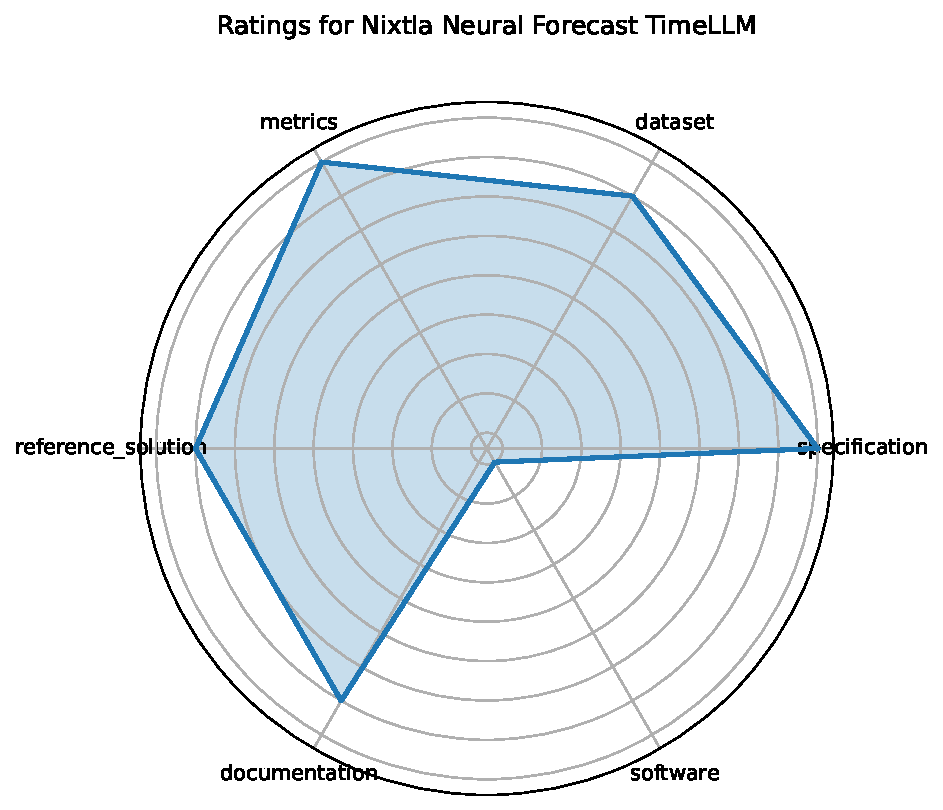
\includegraphics[width=0.7\textwidth]{Nixtla Neural Forecast TimeLLM_radar.pdf}
  \caption{Nixtla Neural Forecast TimeLLM}
\end{figure}

\begin{figure}[h!]
  \centering
  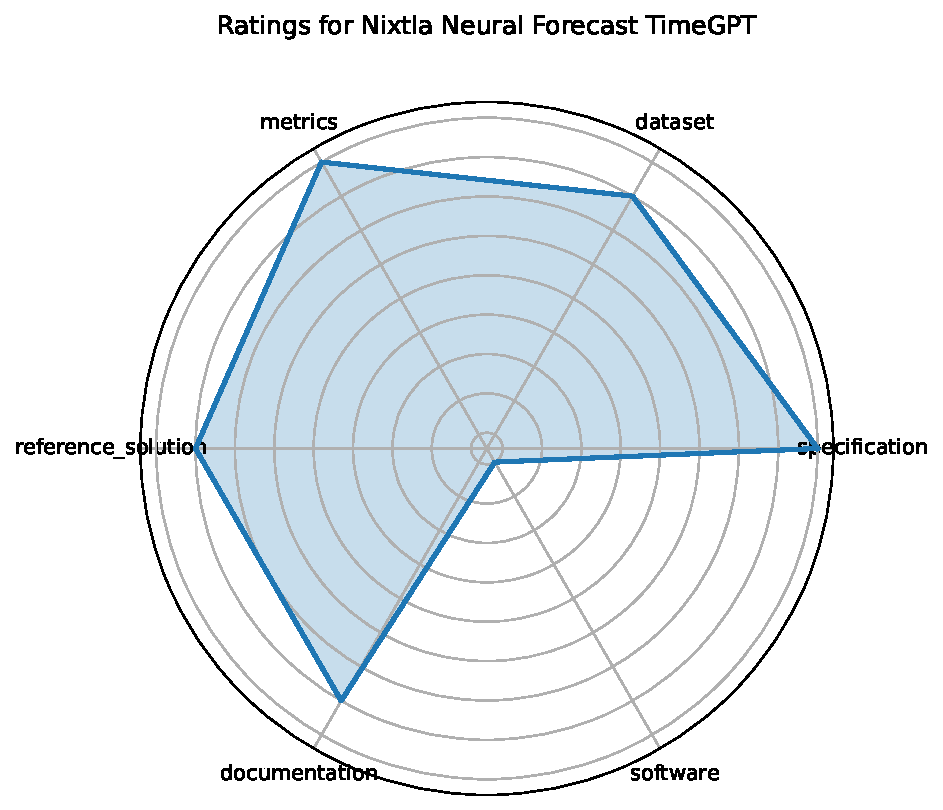
\includegraphics[width=0.7\textwidth]{Nixtla Neural Forecast TimeGPT_radar.pdf}
  \caption{Nixtla Neural Forecast TimeGPT}
\end{figure}

\begin{figure}[h!]
  \centering
  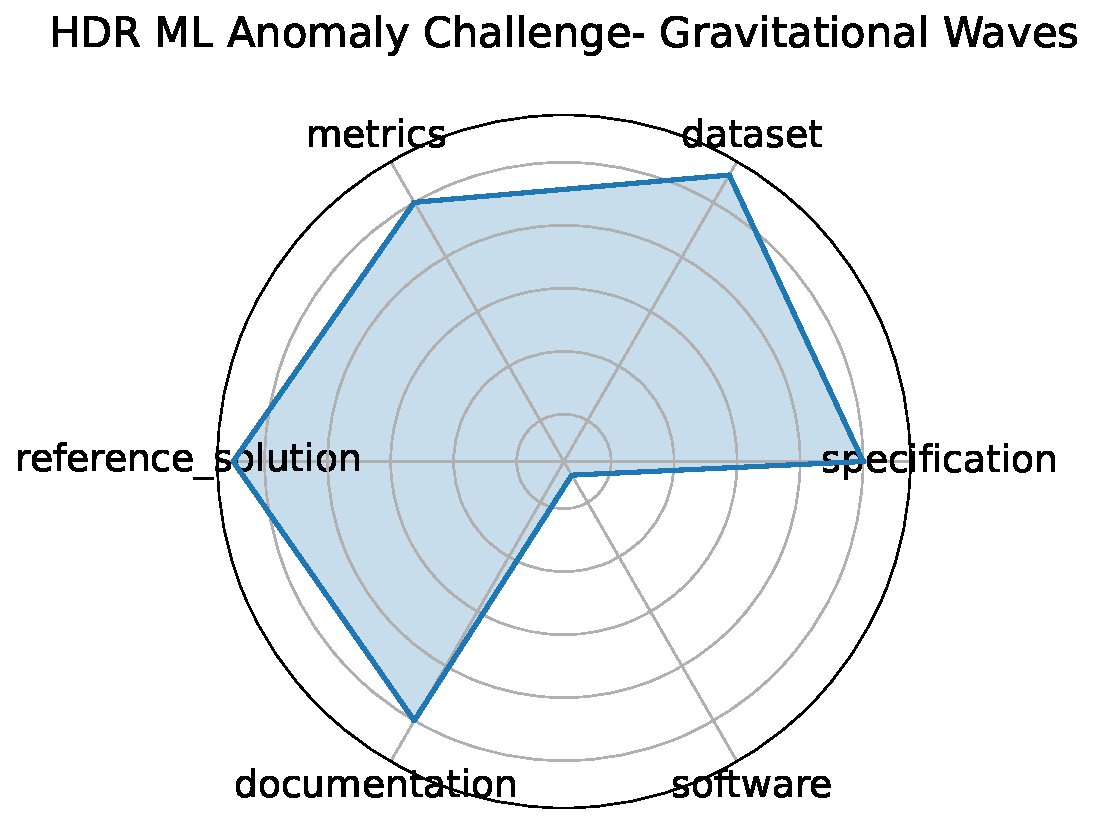
\includegraphics[width=0.7\textwidth]{HDR ML Anomaly Challenge- Gravitational Waves_radar.pdf}
  \caption{HDR ML Anomaly Challenge- Gravitational Waves}
\end{figure}

\begin{figure}[h!]
  \centering
  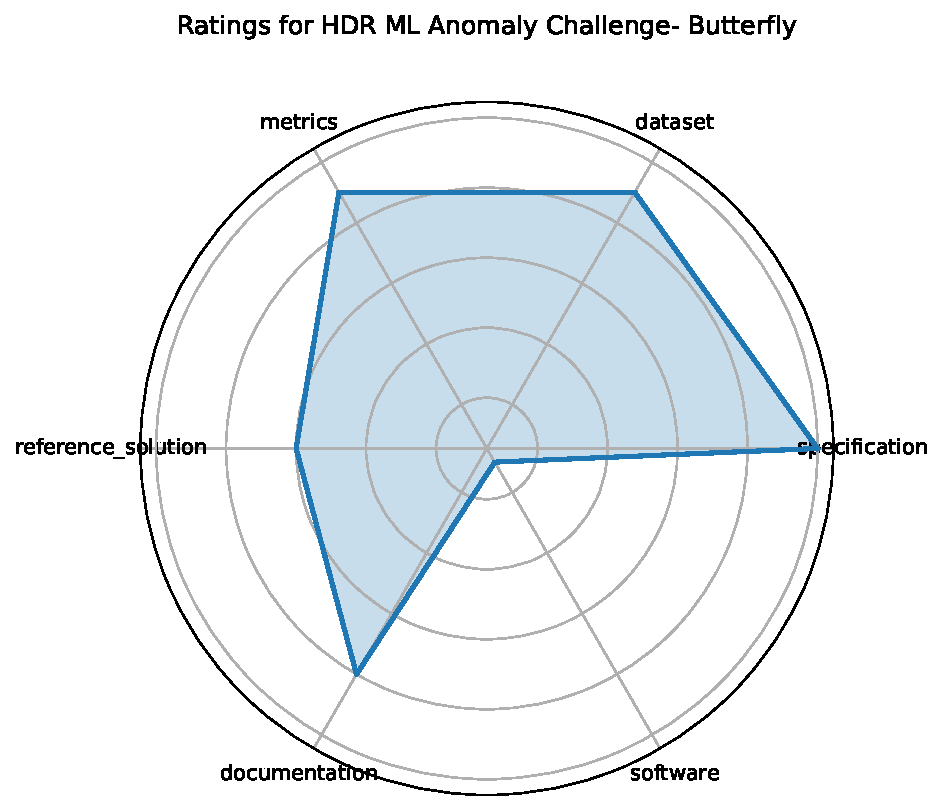
\includegraphics[width=0.7\textwidth]{HDR ML Anomaly Challenge- Butterfly_radar.pdf}
  \caption{HDR ML Anomaly Challenge- Butterfly}
\end{figure}

\begin{figure}[h!]
  \centering
  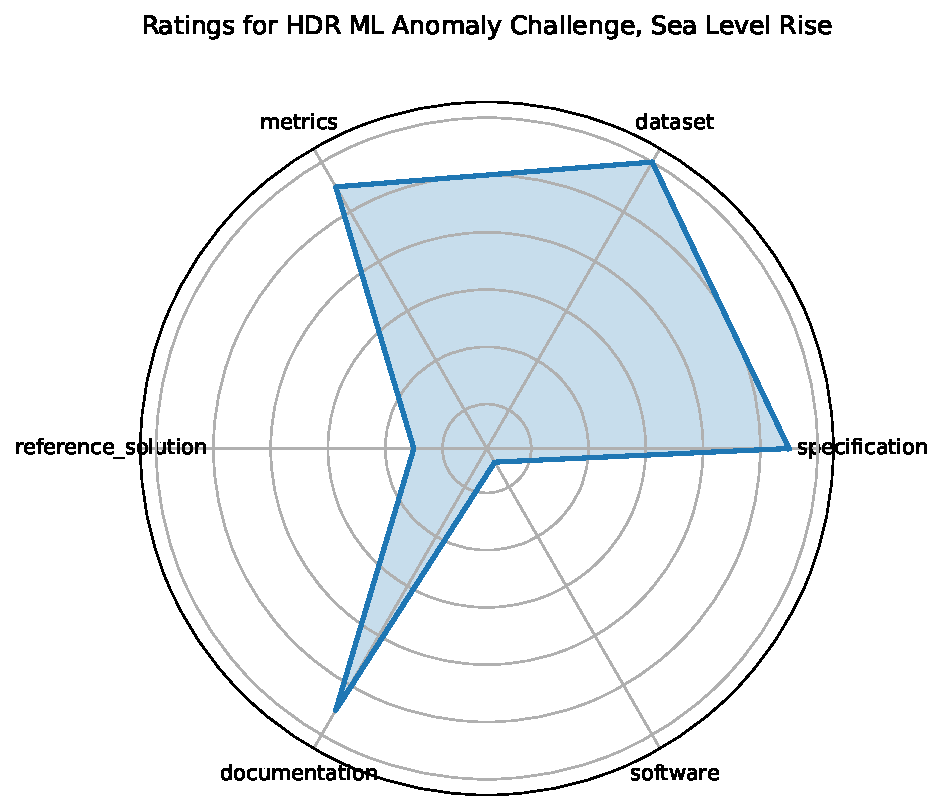
\includegraphics[width=0.7\textwidth]{HDR ML Anomaly Challenge_ Sea Level Rise_radar.pdf}
  \caption{HDR ML Anomaly Challenge, Sea Level Rise}
\end{figure}

\begin{figure}[h!]
  \centering
  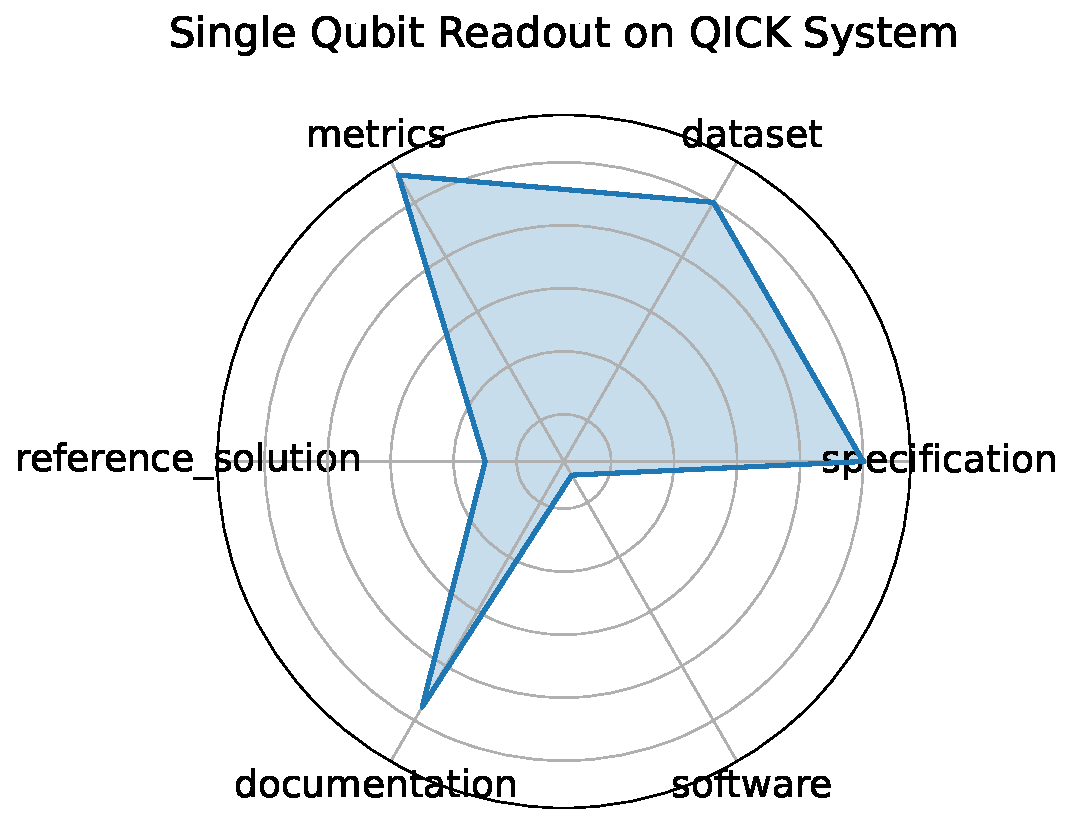
\includegraphics[width=0.7\textwidth]{Single Qubit Readout on QICK System_radar.pdf}
  \caption{Single Qubit Readout on QICK System}
\end{figure}

\begin{figure}[h!]
  \centering
  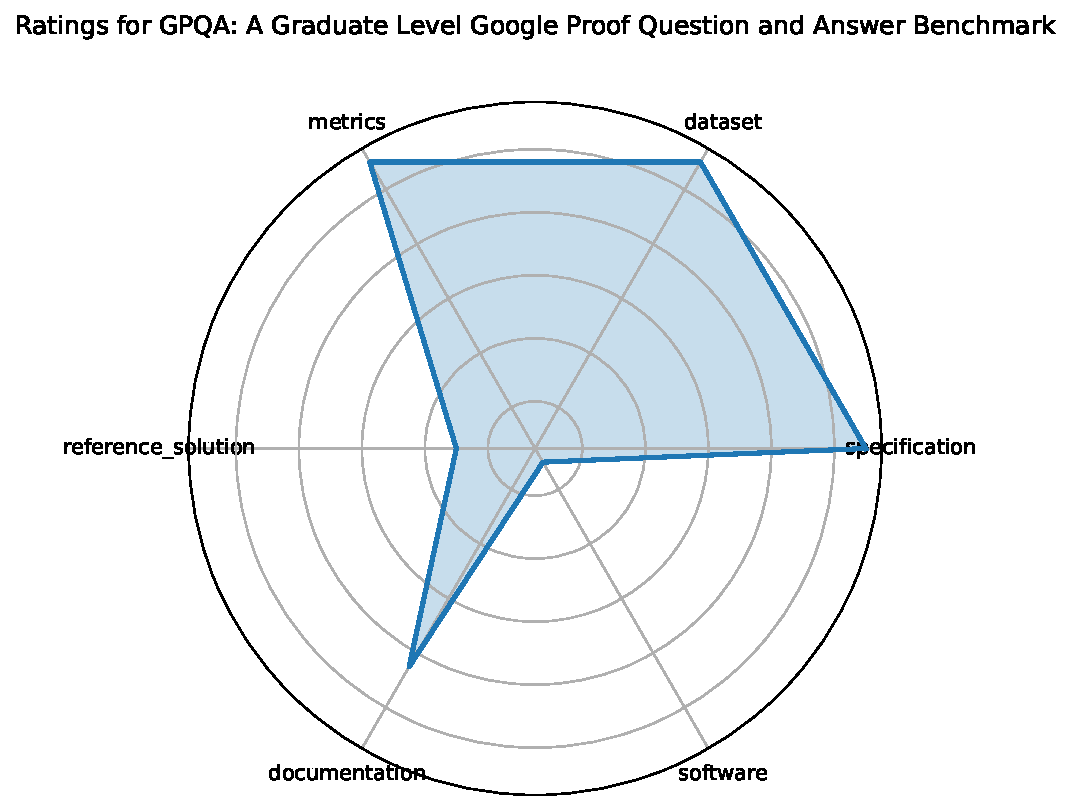
\includegraphics[width=0.7\textwidth]{GPQA_ A Graduate Level Google Proof Question and Answer Benchmark_radar.pdf}
  \caption{GPQA: A Graduate Level Google Proof Question and Answer Benchmark}
\end{figure}

\begin{figure}[h!]
  \centering
  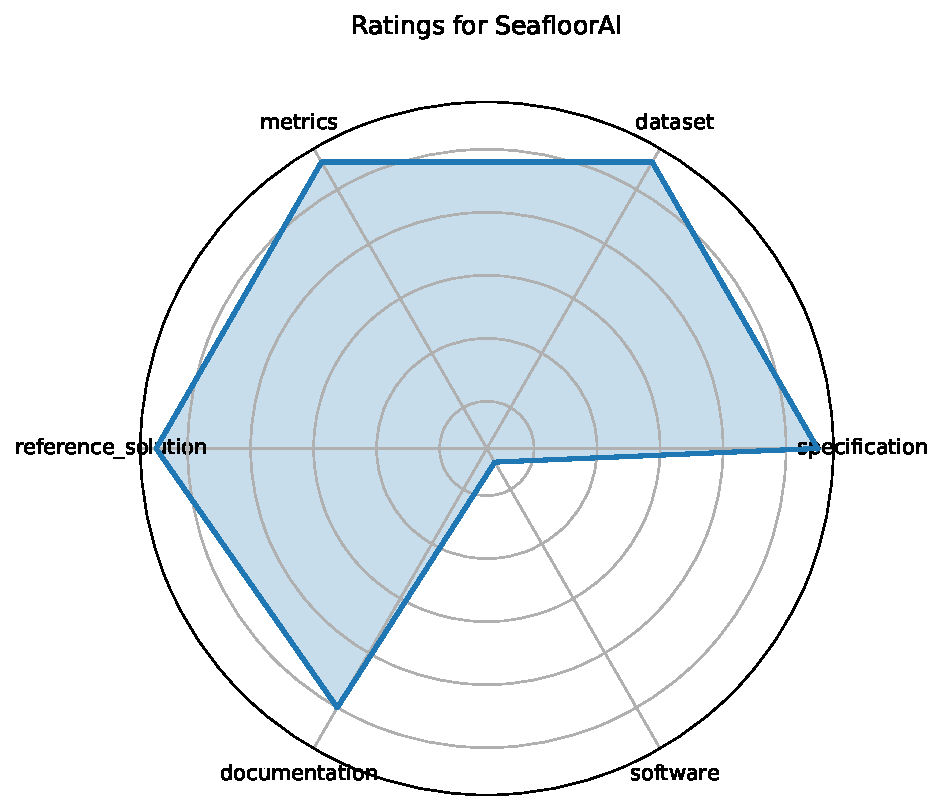
\includegraphics[width=0.7\textwidth]{SeafloorAI_radar.pdf}
  \caption{SeafloorAI}
\end{figure}

\begin{figure}[h!]
  \centering
  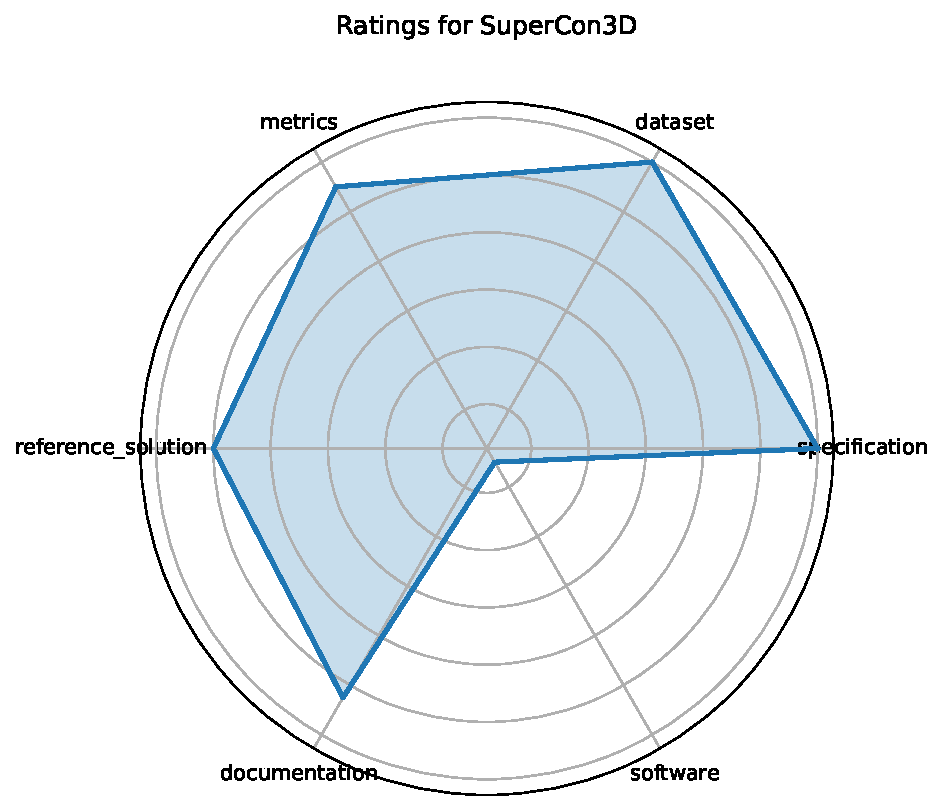
\includegraphics[width=0.7\textwidth]{SuperCon3D_radar.pdf}
  \caption{SuperCon3D}
\end{figure}

\begin{figure}[h!]
  \centering
  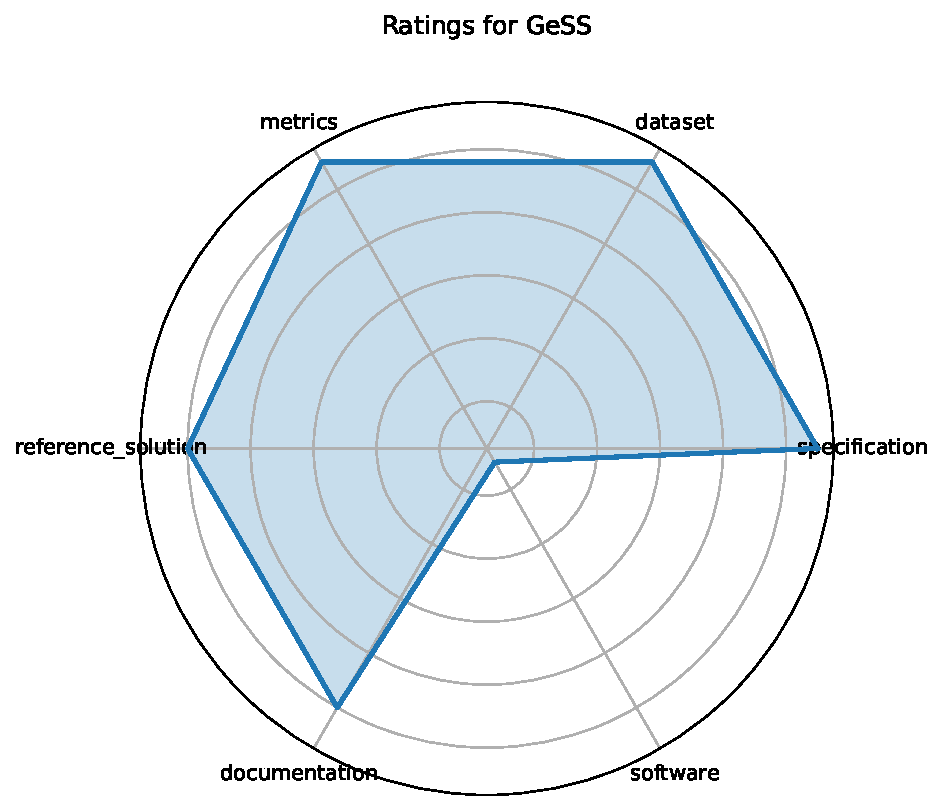
\includegraphics[width=0.7\textwidth]{GeSS_radar.pdf}
  \caption{GeSS}
\end{figure}

\begin{figure}[h!]
  \centering
  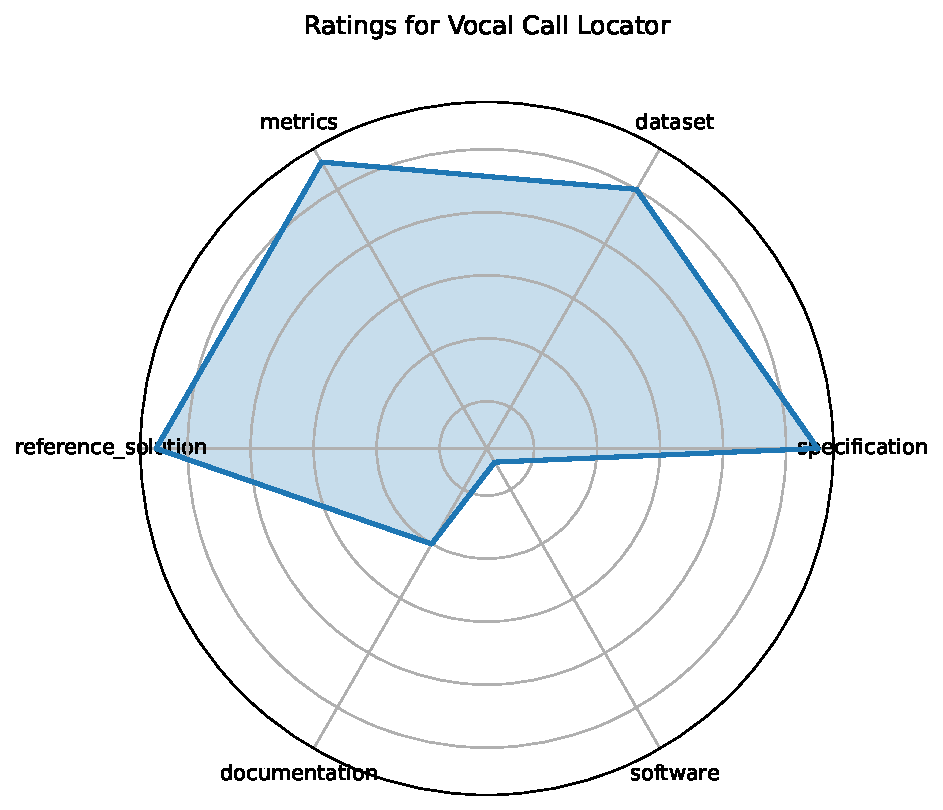
\includegraphics[width=0.7\textwidth]{Vocal Call Locator_radar.pdf}
  \caption{Vocal Call Locator}
\end{figure}

\begin{figure}[h!]
  \centering
  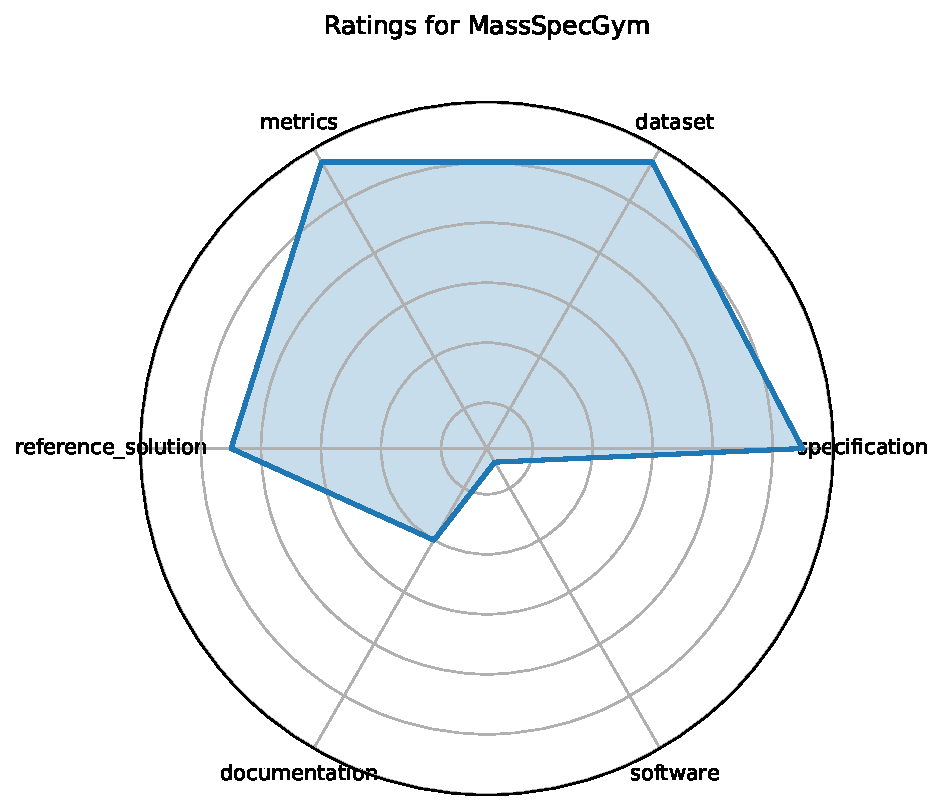
\includegraphics[width=0.7\textwidth]{MassSpecGym_radar.pdf}
  \caption{MassSpecGym}
\end{figure}

\begin{figure}[h!]
  \centering
  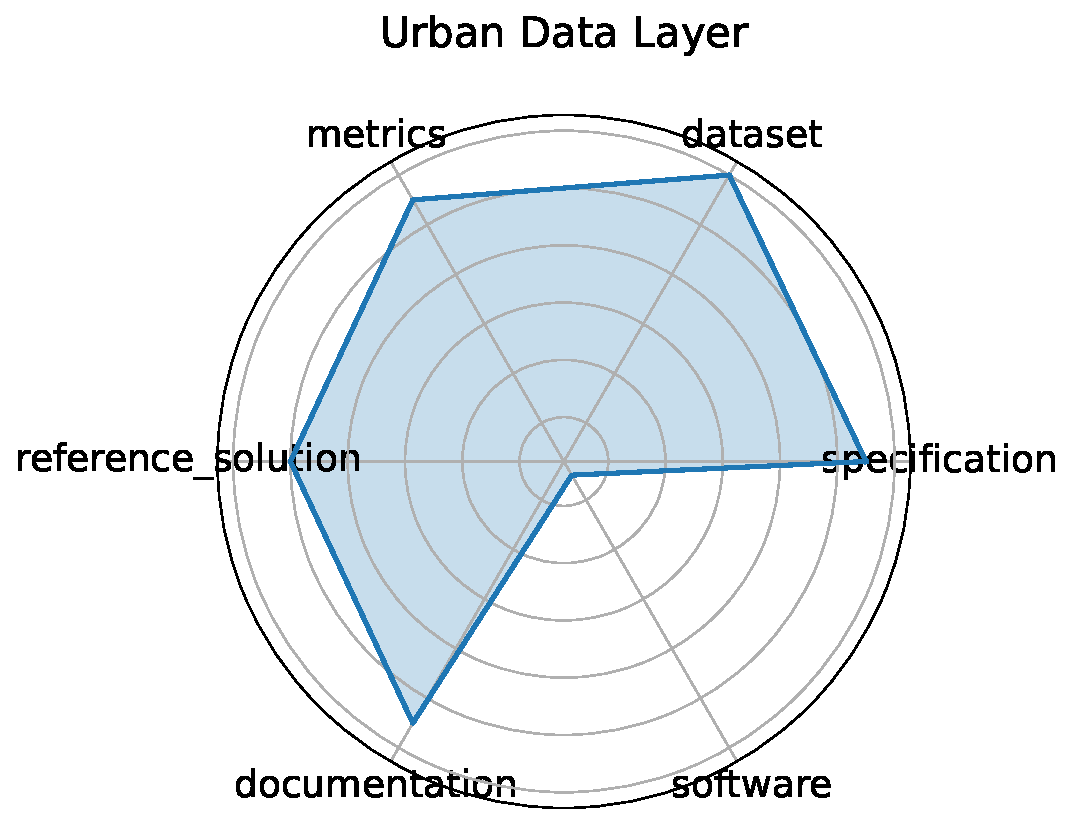
\includegraphics[width=0.7\textwidth]{Urban Data Layer_radar.pdf}
  \caption{Urban Data Layer}
\end{figure}

\begin{figure}[h!]
  \centering
  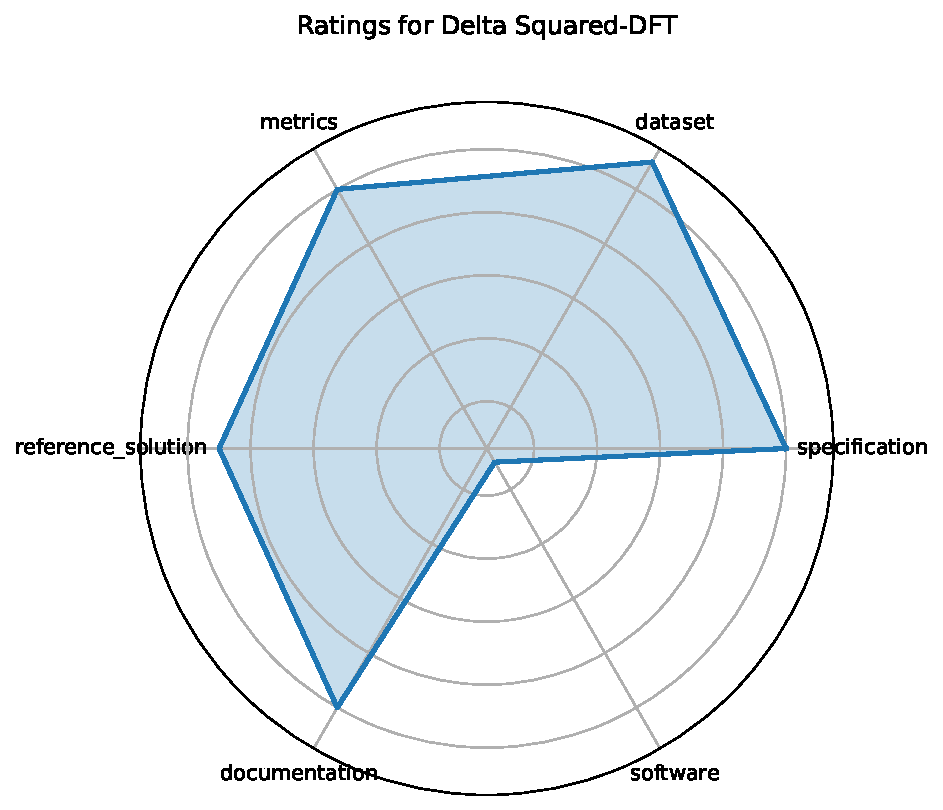
\includegraphics[width=0.7\textwidth]{Delta Squared-DFT_radar.pdf}
  \caption{Delta Squared-DFT}
\end{figure}

\begin{figure}[h!]
  \centering
  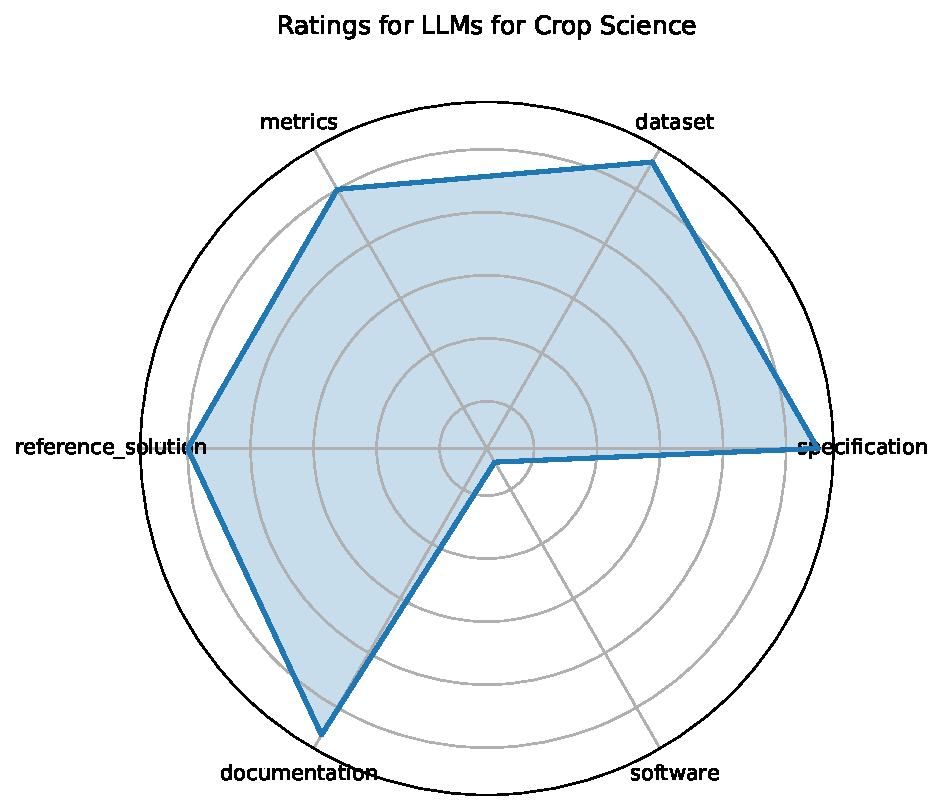
\includegraphics[width=0.7\textwidth]{LLMs for Crop Science_radar.pdf}
  \caption{LLMs for Crop Science}
\end{figure}

\begin{figure}[h!]
  \centering
  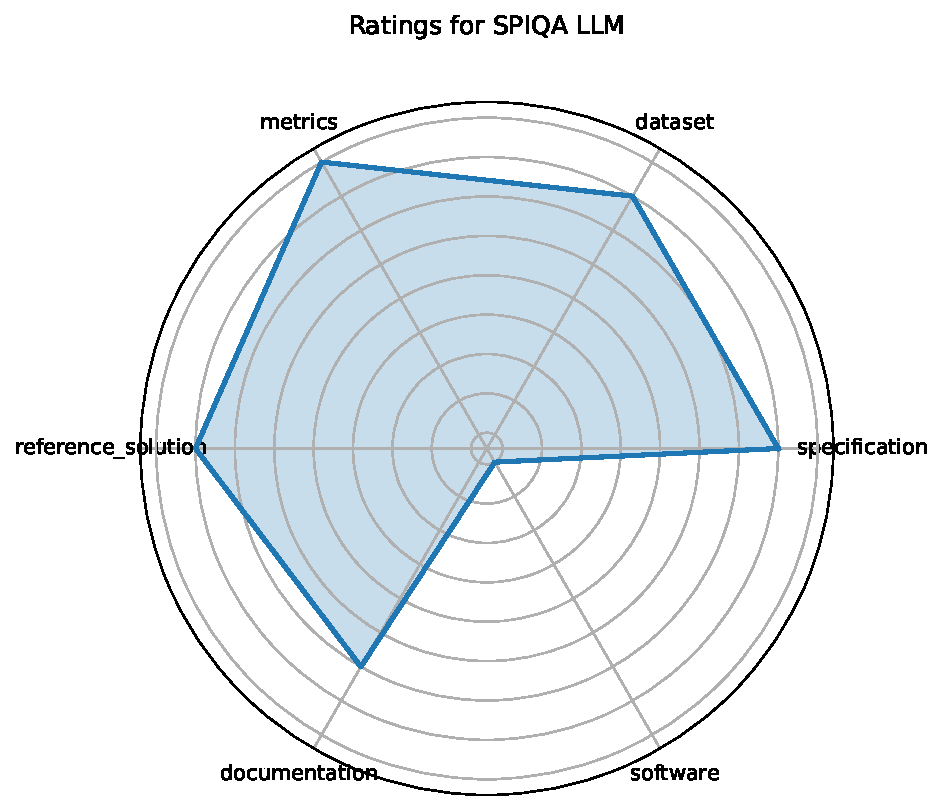
\includegraphics[width=0.7\textwidth]{SPIQA LLM_radar.pdf}
  \caption{SPIQA LLM}
\end{figure}

\end{document}